\section{Variable Metric Bundle Method}
\label{sec_variable_metric}

%\textcolor{red}{can I call this variable metric method or does this imply variable metric updates and not solving the bundle subproblem?}
%\textcolor{blue}{introduction}

A way to extend the proximal bundle method is to use an arbitrary metric \(\frac{1}{2}\Langle d,W_kd \Rangle\) with a symmetric and positive definite matrix \(W_k\) instead of the Euclidean metric for the stabilization term \(\frac{1}{2t_k}\|d\|^2\). Methods doing so are called \emph{variable metric bundle methods}.
This section combines the method of Hare et al. presented in section \ref{sec_nonconv_inex} with the second order model function used by Noll in \cite{Noll2013} to a metric bundle method suitable for nonconvex functions with noise.

The section starts by explaining the ideas from \cite{Noll2013} used to extend the method presented above. It then gives a convergence proof for the developed method and concludes with an explicit strategy how to update the metric during the steps of the algorithm.

Throughout this section we still consider the optimization problem (\ref{opt_prob_nonconv_inex}). We also keep the names and definitions of the objects used in section \ref{sec_nonconv_inex}.

\subsection{Main Ingredients to the Method}
%\textcolor{blue}{explanation}

As already mentioned in section \ref{sec_basic_bundle} the stabilization term can be interpreted in many different ways. In the context of this section we can understand it as a pretty rough approximation of the curvature of the objective function.
In this thesis we work with locally Lipschitz continuous functions. Rademacher's theorem \cite[Theorem 3.1, p. 18]{Heinonen2004} states that on any open set \(U \subset \R^n\) such a function is differentiable at almost every point in \(U\). The set of points where the function is nondifferentiable is of zero Lebesgue measure.
This means that between those points curvature information can be present and can be used to speed up convergence.

%Of course bundle methods are designed to work with non differentiable objectives so it cannot be expected that the function provides any kind of curvature. However, if it has regions where there is curvature, this information can be used to speed up convergence.

\subsubsection{Variable Metric Bundle Methods}

Variable metric bundle methods use an approach that can be motivated by the thoughts stated above.
Instead of using the Euclidean norm for the stabilization term \(\frac{1}{2t_k}\|d\|^2 \) the metric is derived from a symmetric and positive definite matrix \(W_k\). As the name of the method suggests, this matrix can vary over the iterations of the algorithm. The subproblem in the \(k\)'th iteration therefore reads 

\begin{equation*}
	\min_{\hat{x}^k+d \in \R^n} M_k(\hat{x}^k+d)+\mathtt{i}_{X}(\hat{x}^k+d)+\frac{1}{2}\Langle d,W_kd \Rangle.
\end{equation*}

As explained in \cite[chapter XV.4]{Lemarechal1994} like (\ref{sub_prob_fin}) this is a Moreau-Yosida regularization of the objective function (on the constraint set), so this subproblem is still strictly convex and has a unique solution. It is however harder to solve especially if the matrices \(W_k\) are no diagonal matrices \cite[p. 594]{Luksan1999}.
In the unconstrained case or for a very simple constraint set the subproblem can be solved by calculating a quasi Newton step. Such a method is presented by Lemar\'{e}chal and Sagastiz\'{a}bal in \cite{Lemarechal1997} for convex functions. Luk\v{s}an and {Vl\v{c}ek} use an algorithm in those lines in \cite{Vlcek2001} which is adapted to a limited memory setting by Haarala et al. in \cite{Haarala2007}.

A challenging question is how to update the matrices \(W_k\). It is important that the updating strategy preserves positive definiteness of the matrices and that the matrices stay bounded. The updates that are used most often are the symmetric rank 1 formula (SR1 update) and the BFGS (Broyden-Fletcher-Goldfarb-Shanno) update. These updates make it possible to assure the required conditions with only little extra effort even in the nonconvex case. Concrete instances of the updates are given in \cite{Vlcek2001} and \cite{Lemarechal1994}.

%stabilization term mimics curvature \(\to\) more sophisticated in variable metric bundle methods \(\to\) explain those; examples \(\to\) Noll also kind of variable metric bundle method 

\subsubsection{Noll's Second Order Model}

In \cite{Noll2012} Noll et al. present a proximal bundle method for nonconvex objective functions. An important ingredient to the method is that not the objective function itself is approximated in the subproblem but a quadratic model of it:

\begin{equation}
	\Phi(x,\hat{x}) = \phi(x,\hat{x})+\frac{1}{2}\Langle x-\hat{x},Q(\hat{x})(x-\hat{x})\Rangle
\end{equation}

The first order model \(\phi(\cdot,\hat{x})\) is convex and possibly nonsmooth. The second order part \(\frac{1}{2}\Langle \cdot-\hat{x},Q(\hat{x})(\cdot-\hat{x})\Rangle\) is quadratic but not necessarily convex.

As the first order part of this model is convex it can be approximated by a cutting plane model just like the objective function in usual convex bundle methods. The subproblem emerging from this approach is

\begin{equation*}
	\min_{\hat{x}^k+d} m_k(\hat{x}^k+d)+\frac{1}{2}\Langle d,Q(\hat{x}^k)d \Rangle + \frac{1}{2t_k}\|d\|^2
\label{sub_prob_Noll}
\end{equation*} 

where \(m_k\) is the usual cutting plane model (\ref{cp_model}) for the convex, nonsmooth function \(\phi\).

The matrix \(Q(\hat{x}^k)\) itself does not have to be positive definite. In fact the only conditions put on this matrix are that it is symmetric and that all eigenvalues are uniformly bounded.
We adopt the notation in \cite{Noll2013} and write

\begin{equation*}
		Q(\hat{x}^k):=Q_k = Q_k^{\top} \quad \text{and} \quad -q\mathbb{I} \preccurlyeq Q_k \preccurlyeq q\mathbb{I} \text{ for a } q  > 0.
\end{equation*}

The notation \( A \preccurlyeq B\) with \(A, B \in \R^{n\times n}\) means that the matrix \((B-A)\) is positive semidefinite. The symbol \(\prec\)  means analogously that \((B-A)\) is positive definite.

As the matrix \(Q_k\) is symmetric it can also be pulled into the stabilization term. This means the \(k\)'th bundle subproblem can also be written as

\begin{equation}
	\min_{\hat{x}^k+d \in X} m_k(\hat{x}^k+d) + \frac{1}{2}\Langle d,\left(Q_k+\frac{1}{t_k}\mathbb{I} \right) d \Rangle.
\end{equation}

During the algorithm it is assured that \(W_k = Q_k+\frac{1}{t_k}\mathbb{I}\) is positive definite, so this is a variable metric subproblem.

Instead of the first order model \(\phi(\cdot,\hat{x})\) the convexified objective function (\ref{conv_obj}) is used. In the subproblem this function is approximated by the augmented cutting plane model \(M_k\) given in (\ref{aug_model}).
The final subproblem of this variable metric bundle algorithm is then

\begin{equation}
	\min_{\hat{x}^k+d \in X} M_k(\hat{x}^k+d) + \frac{1}{2}\Langle d,\left(Q_k+\frac{1}{t_k}\mathbb{I} \right) d \Rangle.
	\label{Q_subprob}
\end{equation}

The decomposition of the stabilization term into a curvature approximation and a proximal term makes is easier to reach two goals at the same time:

One the one hand, curvature of the objective can be approximated only under the conditions of the boundedness and symmetry of \(Q_k\). No positive definiteness has to be ensured for convergence.
On the other hand the proximal term can be used in the trust region inspired way to make a line search obsolete. As already mentioned in section \ref{sec_simplifications} this is an advantage especially when working with inexact functions where a line search is not useable.

\textcolor{red}{comment on line search and curve search in \cite{Lemarechal1994,Lemarechal1997,Vlcek2001}?}

\subsubsection{The Descent Measure}

%There are some minor changes that have to be made compared to the algorithm proposed by Hare et al. the biggest being the descent measure \(\delta_k\).
Due to the different formulation of subproblem (\ref{Q_subprob}) the descent measure \(\delta_k\) has to be adapted in the variable metric bundle method.
In the same way as for (\ref{agg_subgr_dk}) from the optimality condition

\begin{align*}
	& 0 \in \partial M_k(x^{k+1})+\partial\mathtt{i}_{X}(x^{k+1})+\left(Q_k+\frac{1}{t_k}\mathbb{I}\right)d^k
	\label{Noll_opt_cond}
\end{align*}

it follows that 
\begin{equation}
	S^k+\nu^k = -\left(Q_k+\frac{1}{t_k}\mathbb{I}\right)d^k,
	\label{subgr_Q}
\end{equation}

\(S^k\) and \(\nu^k\) being the augmented aggregate subgradient and outer normal defined in (\ref{aug_agg_subgr}) and (\ref{nu}) respectively.

From this the model decrease (\ref{mod_dec2}) can be calculated using (\ref{aug_agg_lin}), (\ref{aug_agg_err2}) and (\ref{subgr_Q}):

\begin{equation}
\begin{split}
	\delta_k  &:= \hat{f}_k - M_k(x^{k+1}) - \Langle\nu^k,d^k\Rangle\\
	&= \hat{f}_k - A_k(x^{k+1}) - \Langle\nu^k,d^k\Rangle\\
	%&= C_k - (S^k)^{\top}d^k - (\nu^k)^{\top}d^k \\
	&= C_k - \Langle S^k+\nu^k,d^k\Rangle \\
	&= C_k + \Langle d^k,\left(Q_k+\frac{1}{t_k}\mathbb{I}\right)d^k\Rangle \quad \forall k \in \N.
	\label{Noll_delta}
\end{split}
\end{equation}

The new \(\delta_k\) is used in the same way as in algorithm \ref{sec_nonconv_inex}.1 for the descent test and stopping conditions.

Because the changes in the algorithm concern only the stabilization and the decrease measure \(\delta_k\) all other relations that were obtained for the different parts of the model \(M_k\) in section \ref{sec_nonconv_inex} are still valid.

\subsection{The Variable Metric Bundle Algorithm}

The variable metric bundle algorithm can now be stated as a variation of algorithm \ref{sec_nonconv_inex}.1.

%\textcolor{red}{same form as Hare algorithm (nullstep)\\
%add \(Q_k\) calculation}

\begin{minipage}\linewidth
\vspace{1em}
\hrule  \vspace{0.4ex} \hrule
\vspace{1ex}
\textbf{Algorithm \ref{sec_variable_metric}.1: Nonconvex Variable Metric Bundle Method with Inexact Information}
\vspace{1ex}
\hrule
\vspace{1ex}
Select parameters \( m \in (0,1), \gamma > 0, q > 0, 0 < t_{min} < \frac{1}{q} \) and a stopping tolerance \( \mathtt{tol} \geq 0\). Choose a starting point \(x^1 \in \R^n\) and compute \(f_1\) and \(g^1\). Set the initial metric matrix \(Q_1 = \mathbb{I}\), the initial index set \(J_1:=\{1\}\) and the initial prox-center to \(\hat{x}^1 := x^1\). Set \(\hat{f}_1 = f_1\), \(s^1_1 = g^1\) and select \(t_1 > 0\). Initialize \(c^1_1 = 0\) and \(M_1(\hat{x}^1+d)=\hat{f}_1+\Langle s^1_1,d\Rangle\).
\end{minipage}

For \(k = 1,2,3,  \dotsc \)   

\begin{enumerate}
	\item Calculate \[d^k = \argmin_{d \in \R^n} \left\{ M_k(\hat{x}^k+d)+\mathtt{i}_X(\hat{x}^k+d)+\frac{1}{2}\Langle d,\left(Q_k+\frac{1}{t_k}\mathbb{I}\right)d\Rangle\right\}.\]
	\item Set %\textcolor{red}{\(\to\) other stopping condition!!!
		\begin{align*} 
		  G^k &= \sum_{j \in J_k}{\alpha_j^k s_j^k}, \\ %, \quad	\nu^k = -\frac{1}{t_k}d^k-G^k???????????\\
			C_k &= \sum_{j \in J_k}{\alpha_j^k c_j^k} \text{ and} \\
	    \delta_k &=  C_k + \Langle d^k,\left(Q_k+\frac{1}{t_k}\mathbb{I}\right)d^k\Rangle.
		\end{align*}
		If \(\delta_k \leq \mathtt{tol} \rightarrow \) STOP.
	\item Set \( x^{k+1} = \hat{x}^k + d^k \).
	\item Compute \(f^{k+1}, g^{k+1}\). \\
	If \(f^{k+1} \leq \hat{f}^k - m\delta_k \quad \rightarrow \) serious step: \\
	\noindent\hspace*{2em}%
	Set \(\hat{x}^{k+1} = x^{k+1}, \hat{f}^{k+1} = {f}^{k+1}\) and calculate a symmetric matrix \(Q_{k+1}\) with \(-q\mathbb{I} \preccurlyeq Q_{k+1} \preccurlyeq q\mathbb{I}\). \\
	Adjust \(t_{k+1}\) such that \(Q_{k+1}+\frac{1}{t_{k+1}}\mathbb{I} \succ 0\) and \(t_{k+1} > t_{min}\).\\
	Otherwise \(\quad \rightarrow\) nullstep: \\
	\noindent\hspace*{2em}%
	Set \(\hat{x}^{k+1} = \hat{x}^k, \hat{f}^{k+1}=\hat{f}^{k}\) and choose \(t_{min} < t_{k+1} \leq t_k\). 	
	\item Select the new bundle index set \(J_{k+1}\). Calculate 
	\[ \eta_{k+1} = \max{\left\{\max_{j \in J_{k+1}, x^j \neq \hat{x}^{k+1}}{\frac{-2e_j^{k+1}}{|x^j - \hat{x}^{k+1}|^2}, 0}\right\}}+\gamma  \]
	and \(c^{k+1}_j \) by (\ref{aug_lin_err}) for all \(j \in J^{k+1}\). Update the model \(M_{k+1}\) such that conditions (\ref{Model_update_1}) and (\ref{Model_update_2}) are fulfilled.
\end{enumerate}
\vspace{1ex}
\hrule

\vspace{1.5em}

\subsection{Convergence Analysis}

In this section the convergence properties of the new method are analyzed. We do this the same way it is done by Hare et al. in \cite{Hare2016}.

In the paper all convergence properties are first stated in \cite[Lemma 5]{Hare2016}. It is then shown that all sequences generated by the method meet the requirements of this lemma which is stated as Lemma \ref{Lemma5} in this thesis.

As neither the stabilization nor the descent test are involved in the proof of Lemma \ref{Lemma5} it is the same as in \cite{Hare2016}.

We prove now that also the variable metric version of the algorithm fulfills all requirements of Lemma \ref{Lemma5}.
The proof is divided into two parts. The first case covers the case of infinitely many serious steps, the second one considers infinitely many null steps after a finite number of serious steps.

%For both proofs the following lemma is needed:

For both proofs the equivalence of norms is used between the Euclidean norm and the norm \(\Vert \cdot \Vert_{Q_k+\frac{1}{t_k}\mathbb{I}}\).
We show here shortly, that the matrix \(Q_k+\frac{1}{t_k}\mathbb{I}\) can be used to define a scalar product which induces the norm \(\Vert \cdot \Vert_{Q_k+\frac{1}{t_k}\mathbb{I}}\).

In order to do this, it is first shown, that the matrix \(Q_k+\frac{1}{t_k}\mathbb{I}\) is bounded.

\begin{proposition}
\label{prop_bounded}
	The matrix \(Q_k+\frac{1}{t_k}\mathbb{I}\) is bounded in the sense that \(\left\Vert Q_k+\frac{1}{t_k}\mathbb{I} \right\Vert_2 < \infty \) for all \(k\) and the spectral norm \(\Vert \cdot \Vert_2\) \cite[Example 5.6.6]{Horn2012}.
	
	This means also that the following relation holds for all vectors \(x\in\R^n\):
	
	\begin{equation}
		\left\Vert\left(Q_k+\frac{1}{t_k}\mathbb{I}\right)x\right\Vert \leq \left\vert q + \frac{1}{t_{min}} \right\vert \Vert x\Vert , \quad \forall k,
		\label{rel_bound}
	\end{equation}
	
	where \(q > 0\) is the bound on the eigenvalues of \(Q_k\) and \(t_{min}\) the lower bound for the step size. \\
	Inequality (\ref{rel_bound}) also holds true in the limit \(k \to \infty\).
\end{proposition}

\begin{proof}
	%To show boundedness of the matrix \(Q_k+\frac{1}{t_k}\mathbb{I}\) we show that the spectral norm of this matrix is bounded.
	
	Algorithm \ref{sec_variable_metric}.1 ensures that \( -q \mathbb{I}  \preccurlyeq Q_k \preccurlyeq q\mathbb{I} \) for some preset constant \(q >0\). This means, that the matrices \(Q_k + q\mathbb{I} \) and \(q \mathbb{I} - Q_k \) are positive semidefinite yielding that all their eigenvalues are nonnegative.
	
In section \ref{proof_eigval} in the appendix it is shown that the eigenvalues of a matrix of the form \(A+b\mathbb{I}\) for a symmetric matrix \(A \in \R^{n\times n}, b \in \R\) are \(\tilde{\lambda}_i := \lambda^A_i+b \), with \(\lambda^A_i\), \(i =1,...,n\) being the eigenvalues of the matrix \(A\).
This means that the following holds for all eigenvalues \(\lambda^k_{i}\), \(i = 1,...,n\), of \(Q_k\), which is symmetric, for all \(k\):

\begin{equation*}
	\lambda^k_{i} + q \geq 0 \text{ and } q - \lambda^k_{i} \geq 0 \quad \Rightarrow \quad \vert \lambda^k_{i} \vert \leq q, \quad  i = 1,...,n, \quad  \forall k.
\end{equation*}
	
	This means that also \(\lim_{k \to \infty} \vert \lambda^k_{i} \vert \leq q\).
	
The step size \(t_k\) is bounded below by \(t_{min}\) for all \(k\) and hence also for \(k \to \infty\). This yields for the spectral norm that

\begin{equation}
		\Vert Q_k+\frac{1}{t_k}\mathbb{I} \Vert_2 =  \vert \lambda^k_{max}+\frac{1}{t_k} \vert \leq \vert q+\frac{1}{t_{min}} \vert < \infty, \quad \forall k.
		\label{bound}
\end{equation}

Here \(\lambda^k_{max}\) denotes the eigenvalue of \(Q_k\)  that fulfills \(\lambda^k_{max} = \argmax_{i \in \{1,...,n\}} \vert \lambda^k_{i}+\frac{1}{t_k} \vert\).

The spectral norm is induced by the Euclidean norm thus it is compatible with it. Therefore with relation (\ref{bound}) it holds

\[ \left\Vert \left(Q_k+\frac{1}{t_k}\mathbb{I}\right)x \right\Vert \leq \left\Vert Q_k+\frac{1}{t_k}\mathbb{I} \right\Vert_2 \Vert x \Vert \leq \left\vert q+\frac{1}{t_{min}} \right\vert \Vert x \Vert , \quad \forall k.\]

The estimates above were also shown to hold in the limit \(k \to \infty\) so the inequalities hold also true in that case. 
\end{proof}



\begin{proposition}
\label{prop_norm}
	The norm \(\Vert \cdot \Vert_{Q_k+\frac{1}{t_k}\mathbb{I}}\) induced by the matrix \(Q_k+\frac{1}{t_k}\mathbb{I}\) is well-defined for all \(k\).
\end{proposition}

The proof to this proposition is found in section \ref{proof_norm} of the appendix.

%\begin{proposition}
	%Under the assumption that the matrix \(Q_k+\frac{1}{t_k}\mathbb{I}\) is uniformly bounded for all \(k\) the expression \(\Vert \cdot \Vert_{Q_k+\frac{1}{t_k}\mathbb{I}}\) defines a norm.
%\end{proposition}
%
%\begin{proof}
	%To proof that \(\Vert \cdot \Vert_{Q_k+\frac{1}{t_k}\mathbb{I}}\) defines a norm the norm axioms are shown for the expression.
	%
	%1. Definiteness: \(\Vert x \Vert_{Q_k+\frac{1}{t_k}\mathbb{I}} = 0 \Rightarrow x = 0\).
	%
	%This follows directly from positive definiteness of the matrix \({Q_k+\frac{1}{t_k}\mathbb{I}}\) because it yields
	%
	%\[\sqrt{\Langle x,\left(Q_k+\frac{1}{t_k}\mathbb{I}\right) x \Rangle} = 0 \quad \Rightarrow \quad x = 0. \]
	%
	%2. Absolute homogeneity: \(\Vert ax \Vert_{Q_k+\frac{1}{t_k}\mathbb{I}} = \vert a \vert \Vert x \Vert_{Q_k+\frac{1}{t_k}\mathbb{I}}\) for \(a \in \R\).
	%
	%This follows from the properties of the scalar product:
	%
	%\[\Vert ax \Vert_{Q_k+\frac{1}{t_k}\mathbb{I}} = \sqrt{\Langle ax,\left(Q_k+\frac{1}{t_k}\mathbb{I}\right)\cdot (ax) \Rangle} = \sqrt{a^2}\Vert x \Vert_{Q_k+\frac{1}{t_k}\mathbb{I}} = \vert a \vert \Vert x \Vert_{Q_k+\frac{1}{t_k}\mathbb{I}}\]
	%
	%3. Triangle inequality: \(\Vert x+y \Vert_{Q_k+\frac{1}{t_k}\mathbb{I}} \leq \Vert x \Vert_{Q_k+\frac{1}{t_k}\mathbb{I}}+\Vert y \Vert_{Q_k+\frac{1}{t_k}\mathbb{I}}\).
	%
	%This follows with the Cauchy-Schwarz inequality and symmetry of \(Q_k+\frac{1}{t_k}\mathbb{I\).
	%
%\begin{align*}
	%\Vert x+y \Vert_{Q_k+\frac{1}{t_k}\mathbb{I}} &= \sqrt{\Langle x+y,\left(Q_k+\frac{1}{t_k}\mathbb{I}\right)\cdot (x+y) \Rangle} \\
	%&= \sqrt{\Langle x,\left(Q_k+\frac{1}{t_k}\mathbb{I}\right)x \Rangle + \Langle y,\left(Q_k+\frac{1}{t_k}\mathbb{I}\right)y \Rangle +2 \Langle x,\left(Q_k+\frac{1}{t_k}\mathbb{I}\right)y \Rangle} \\
	%& \leq \sqrt{\Vert x \Vert_{Q_k+\frac{1}{t_k}\mathbb{I}}^2 + \Vert y \Vert_{Q_k+\frac{1}{t_k}\mathbb{I}}^2+2
%\end{align*}
	%
%\end{proof}

%\begin{lemma}
	%For a symmetric matrix \(A \in \R^{n\times n}\), a vector \(d\in \R^n\) and \(\xi > 0\) the following result holds: 
	%\[ A \prec \xi \mathbb{I} \Rightarrow Ad < \xi d. \]
	
	%The second inequality is meant componentwise.
%\end{lemma}

%\begin{proof}
	%As the matrix \(A\) is real and symmetric it is orthogonally diagonalizeable.
	%There exist eigenvalues \(\lambda_i \in \R, i = \{1,...,n\}\) and corresponding eigenvectors \(v^i \in \R^n, i = \{1,...,n\}\) that satisfy the equations
	%
	%\begin{equation*}
		%Av^i= \lambda_iv^i \quad i = \{1,...,n\}.
		%\label{A_d_rel}
	%\end{equation*}
	%
	%The eigenvectors \(v^i\) generate a basis for \(\R^n\) so any vector \(d \in \R^n\) can be written as
	%
	%\[ d = \sum_{i} {\alpha_i v^i} \]
	%
	%for \(\alpha_i \in \R^n, i = \{1,...,n\}\).
	%
	%This yields
	%
	%\begin{equation}
		%Ad = A \sum_i{\alpha_i v^i} = \sum_i \alpha_i \lambda_i v^i.
		%\label{Ad}
	%\end{equation}
	%
	%Plugging the assumption \(A \prec \xi \mathbb{I}\) which is equivalent to \(\max_i \lambda_i < \xi\) into (\ref{Ad})
	%%we get relation (\ref{A_d_rel}) by
	%	%\[Ad < \xi \sum_i \alpha_i v^i = \xi d. \]
%
	%%\[ A \succ B \Leftrightarrow A - B \succ 0\Leftrightarrow A-B \text{ is positive definite}\]
	%%Respectively for \(A \prec B\) \\
%\end{proof}

The first part of the convergence proof is now stated.

\begin{theorem}[c.f. {\cite[Theorem 6, p. 14]{Hare2016}}]
\label{theo_inf_ser_steps}
	%\(\to\) take only part with \(\liminf_{k\to\infty}t_k > 0 \) because other one not used in null steps and algorithm this way. \\
	Let algorithm \ref{sec_variable_metric}.1 generate an infinite number of serious steps. Then \(\delta_k \to 0\) as \(K \ni k \to \infty\) for the sequence of serious steps \(K \subset \{1,2,...\}\). 
	Let the sequence \(\{\eta_k\}\) be bounded. As \(K \ni k \to \infty\) we have \(C_k \to 0\). For every accumulation point \(\bar{x}\) of \(\{\hat{x}^k\}\) there exists a subsequence \(\tilde{K}\) and  a vector \(\bar{S}\) such that \(S^{\tilde{k}} \to \bar{S}\) and \(S^{\tilde{k}} + \nu^{\tilde{k}} \to 0\) for \(\tilde{K} \ni \tilde{k} \to \infty\).
In particular if the cardinality of \(\{j \in J^k\mid \alpha_j^k > 0\}\) is uniformly bounded in \(k\) then the conclusions of Lemma \ref{Lemma5} hold.
\end{theorem}

The proof is very similar to the one stated in \cite{Hare2016} but minor changes have to be made due to the different formulation of the nominal decrease \(\delta_k\).

\begin{proof}
	Let \(K \subset \{1,2,...\}\) denote the subsequence of serious steps. (For the sake of readability the same index \(k\) that is used in the algorithm for all steps is used here only for the serious steps.)
	At each of those steps we have
	
	\begin{equation}
		\hat{f}_{k+1} \leq \hat{f}_k - m\delta_{k}, \quad {k} \in {K} 
	\label{nonincreasing}
	\end{equation}
	
	where \(m, ~\delta_{k} > 0\). 
	As \(\hat{f}_k\) is only updated in serious steps it follows that the sequence \(\{\hat{f}_k\}\) is nonincreasing.
	Since the sequence \(\{\hat{x}^k\}\) lies in the compact set \(X\) and \(f\) is continuous the sequence \(\{f(\hat{x}^k)\}\) is bounded. %\textcolor{red}{which assumption says \(f\) bounded below??? \(\to\) \(f\) subdifferentially regular \(\Rightarrow\) \(f\) finite}
	With \(|\sigma_k| < \bar{\sigma}\) also the sequence \(\{f(\hat{x}^k)+\sigma_k\} = \{\hat{f}_k\}\) is bounded. Considering also the fact that \(\{\hat{f}_k\}\) is nonincreasing one can conclude that it converges. \\
	From (\ref{nonincreasing}) follows that
	
	\begin{equation*}
		0 \leq m \sum_{k = 1}^l \delta_k \leq \sum_{k = 1}^l \left(\hat{f}_k-\hat{f}_{k+1}\right),
	\end{equation*}
	
	so letting \(l \to \infty\), 
	
	\begin{equation*}
		0 \leq m\sum_{k=1}^{\infty} \delta_k \leq \hat{f}_1 - \underbrace{\lim_{k \to \infty} \hat{f}_k}_{\neq \pm \infty}.
	\end{equation*}
	
	This yields
	\begin{equation*}
		\sum_{k = 1}^{\infty} \delta_k = \sum_{k=1}^{\infty}\left(C^k+\Langle d^k,\left(Q_k+\frac{1}{t_k}\mathbb{I}\right)d^k\Rangle \right) < \infty.
	\end{equation*}
	
	Hence, \(\delta_k \to 0\) as \(k \to \infty\). All quantities above are nonnegative due to positive definiteness of \(Q_k+\frac{1}{t_k}\mathbb{I}\) and \(C_k \geq 0\) so it also holds that
	
	\begin{equation*}
		C_k \to 0 \quad \text{and} \quad \Langle d^k,\left(Q_k+\frac{1}{t_k}\mathbb{I}\right)d^k\Rangle \to 0.
	\end{equation*}
	
	Finally we need to show that for any accumulation point \(\bar{x}\) of the sequence \(\{\hat{x}^{\tilde{k}}\}\) holds \(S^{\tilde{k}} \to \bar{S}\) and \(S^{\tilde{k}}+\nu^{\tilde{k}} \to 0\) for \(\tilde{K} \ni {\tilde{k}} \to \infty\) and the suitable subsequence \(\tilde{K} \subset K\).
Let \({K'} \subset K\) denote the subset such that the sequence \(\{\hat{x}^{k'}\}\) converges to its accumulation point \(\bar{x}\) for \(k' \in K'\). %Let then \(\hat{K'} \subset K'\) be the subset of iterates where serious steps were done. 
As we only consider the subsequence of serious steps it follows from \(\{\hat{x}^{k'}\}_{k' \in K'} \to \bar{x}\) that  \(d^{{k'}} = \hat{x}^{{k'}+1}-\hat{x}^{{k'}} \to 0\) for \({K'} \ni {k'} \to \infty \). The step size \(t_k\) is bounded below by \(t_{min} > 0\) and because the eigenvalues of \(Q_k\) are bounded the expression 
	
	\begin{equation*}
	 S^{{k'}} + \nu^{{k'}} = \left(Q_{{k'}}+\frac{1}{t_{{k'}}}\mathbb{I} \right)d^{{k'}}  \to 0 \quad \text{for} \quad {K'} \ni {k'} \to \infty
	\end{equation*}
	
	because 
	
	\[ \lVert S^{{k'}} + \nu^{{k'}} \rVert = \left\Vert\left(Q_{{k'}}+\frac{1}{t_{{k'}}}\mathbb{I}\right)d^{{k'}} \right\Vert \leq \left \vert q + \frac{1}{t_{min}}\right\vert \underbrace{\|d^{{k'}}\|}_{\to 0}.\]
	
	Here the last inequality follows from (\ref{rel_bound}).
	The implication \(S^{\tilde{k}} \to \bar{S}\) for \({\tilde{k}} \in \tilde{K}\) follows from local Lipschitz continuity of \(f\).
	By Rademacher's theorem this property yields that on any open set \(\Omega\) the function \(f\) is differentiable except on a set \(\Omega_{\text{nd}}\) of zero Lebesgue measure. As \(f\) is also Lipschitz continuous on any closed set containing such an open set \(\Omega\), the gradient of \(f\) on \(\Omega\) is bounded.
	Let \(X \subset \Omega\). By theorem 2.5.1 in \cite[p. 63]{Clarke1990} the subdifferential of \(f\) at any point \(x^k \in \Omega\) is the convex hull of the limits of gradients \(\nabla f\) of \(f\) on the set \(\Omega\setminus \Omega_{\text{nd}}\)
	
		\[ \partial f(x^k) = \conv\{\lim \nabla f(y) \mid y \to x^k, y \notin \Omega_{\text{nd}}\}. \]
		
		This means that also all subgradients on \(\Omega\) are bounded. As the subgradient error is assumed to be bounded by \(\bar{\theta}\) the set of approximate subgradients \(\{g^j, j \in J^k\}\) contained in the bundle is bounded as well.
		From this follows that also the augmented subgradients \(s_j^k = g^j+\eta_k(x^j-\hat{x}^k)\) are bounded because \(\eta^k\) is bounded by assumption and \(x^j, \hat{x}^k \in X\).		
Defining \(s:= \max_{k,j}\|s^k_j\|\) this yields that 
		
		\[\Vert S^k\Vert = \bigg\Vert\sum_{j \in J^k}{\alpha_j^k s_j^k}\bigg\Vert \leq  \sum_{j \in J^k}{\Vert\alpha_j^k\Vert\underbrace{\Vert s^k_j\Vert}_{\leq s \in \R}} \leq s\underbrace{\sum_{j \in J^k}{\alpha_j^k}}_{=1} < \infty \quad \forall k. \]
		
		It follows that the sequence \(S^k\) is bounded.
		By the Bolzano-Weierstrass theorem \cite[p. 51]{Koenigsberger2003} every bounded sequence has a convergent subsequence. Let \(\tilde{K} \subset \hat{K'}\) denote the index set of this converging subsequence and \(\bar{S}\) the corresponding accumulation point. Then finally \(S^{\tilde{k}} \to \bar{S}\) for \(\tilde{K} \ni {\tilde{k}}\to \infty\).
		
	
\end{proof}

%\begin{remark}
%If one assumes that the set \(\Omega = \{x \in \R^n |f(x) \leq f(x^1) +2\bar{\sigma}\}\) is bounded, it is not necessary to use the constraint set \(X\). \\
%Because \(\{\hat{x}^k\} \subset \Omega\) one can deduce the boundedness of the sequence.
%\end{remark}

For the case that only finitely many serious steps are executed we need the following result:

%It only depends on the definitions of the augmented linearization error and subgradient and can therefore be taken without any adaption.

Whenever \(x^{k+1}\) is as declared a null step, a simple calculation shows that the relation 

\begin{equation}
	-c^{k+1}_{k+1} + \Langle s^{k+1}_{k+1}, x^{k+1}-\hat{x}^k\Rangle = f_{k+1}-\hat{f}_k + \underbrace{\frac{\eta_{k+1}}{2}\Vert x^{k+1}-\hat{x}^{k}\Vert^2}_{\geq 0}>-m\delta_k
\label{no_ls}
\end{equation}

holds.
The exact derivation of (\ref{no_ls}) is also given in \cite[p. 16]{Hare2016}.

Another relation that is used a few times throughout the proof is the estimate

\begin{equation}
	\Langle \nu^k, d^k \Rangle \geq 0.
\label{subgr_ineq}
\end{equation}

It follows from the subgradient inequality for the convex function \(\mathtt{i}_X\) at the point \(x^{k+1}\). As \(\nu^k \in \partial \mathtt{i}_X(x^{k+1})\) it holds \(\mathtt{i}_X(y)-\mathtt{i}_X(x^{k+1}) \geq \Langle\nu^k,y-x^{k+1}\Rangle\) for all \(y \in X\) and as \(d^k = x^{k+1}-\hat{x}^k\) and \(x^{k+1}, \hat{x}^k \in X\) it follows

\[ 0 = \underbrace{\mathtt{i}_X(\hat{x}^k)}_{=0} - \underbrace{\mathtt{i}_X(x^{k+1})}_{=0} \geq \Langle \nu^k,\hat{x}^k-x^{k+1}\Rangle = -\Langle \nu^k,d^k\Rangle \]

yielding inequality (\ref{subgr_ineq}) above.


\begin{theorem} [c.f. {\cite[Theorem 7, p. 16]{Hare2016}}]
	Let a finite number of serious iterates be followed by infinite null steps. Let the sequence \(\{\eta_k\}\) be bounded.
	Then \(\{x^k\} \to \hat{x}\), \(\delta_k \to 0\), \(C_k \to 0\), \(S^k + \nu^k \to 0\) and there exist \(K\subset \{1,2,...\}\) and \(\bar{S}\) such that \(S^k \to \bar{S}\) as \(K \ni k \to \infty\). \\
	In particular if the cardinality of \(\{j \in J^k\mid \alpha_j^k > 0 \}\) is uniformly bounded in \(k\) then the conclusions of Lemma \ref{Lemma5} hold for \(\bar{x} = \hat{x}\). 
\end{theorem}

\begin{proof}
	Let \(k\) be large enough such that \(k \geq \bar{k}\), where \(\bar{k}\) is the iterate of the last serious step. Let \(\hat{x}:= \hat{x}^{\bar{k}} \) and \(\hat{f}:= \hat{f}_{\bar{k}}\) be fixed. The matrix \(Q_k\) is also fixed and denoted as \(Q := Q_{\bar{k}}\).
	Define the optimal value of the \(k\)'th subproblem  (\ref{Q_subprob}) for \(k > \bar{k}\) by 
	
	\begin{equation}
		\Psi_k := M_k(x^{k+1})+\frac{1}{2}\Langle d^k,\left(Q+\frac{1}{t_k}\mathbb{I}\right)d^k\Rangle.
		\label{Psi}
	\end{equation}
	
	It is first shown that the sequence \(\{\Psi_k\}\) is bounded above.
	From definition (\ref{aug_agg_lin}) and relation (\ref{A_leq_M}) follows

%\begin{equation*}	
	%A_k(\hat{x}+d) := M_k(x^{k+1})+\Langle S^k,d-d^k\Rangle
	%\label{Noll_agg_lin}
%\end{equation*}
	%of the aggregate linearization follows
	
	\begin{equation*}
		A_k(\hat{x}) = M_k(x^{k+1})-\Langle S^k,d^k \Rangle \leq M_k(\hat{x}).
		%\label{agg_lin_2}
	\end{equation*}
	
Using (\ref{subgr_Q}) for the third equality and (\ref{subgr_ineq}) in the first inequality one obtains
	
	\begin{align*}
		\Psi_k+\frac{1}{2}\Langle d^{k},\left(Q+\frac{1}{t_k}\mathbb{I}\right)d^k\Rangle &= A_k(\hat{x})+\Langle S^k,d^k\Rangle + \Langle d^{k},\left(Q+\frac{1}{t_k}\mathbb{I}\right)d^k\Rangle \\
		&= A_k(\hat{x}) + \Langle S^k + \langle Q+\frac{1}{t_k}\mathbb{I},d^k \rangle,d^k \Rangle \\
		&= A_k(\hat{x})-\Langle \nu^k,d^k \Rangle \\
		&\leq A_k(\hat{x}) \\
		&\leq M_k(\hat{x}) \\
		&= \hat{f}.
	\end{align*}
	
By boundedness of \(d^k\) and boundedness and positive definiteness \(Q+\frac{1}{t_k}\mathbb{I}\) this yields that \(\Psi_k \leq \Psi_k + \frac{1}{2} \Vert d^k\Vert^2_{Q+\frac{1}{t_k}\mathbb{I}} \leq \hat{f}\), so the sequence \(\{\Psi_k\}\) is bounded above.
	In the next step it is shown that \(\{\Psi_k\}\) is increasing. By noting that \(x^{k+2} = \hat{x}+d^{k+1}\), as the proximal center does not change in the null step case, we obtain
	
\begin{equation}
\begin{split}
		\Psi_{k+1} &= M_{k+1}(x^{k+2})+\frac{1}{2}\Langle d^{k+1},\left(Q+\frac{1}{t_{k+1}})\mathbb{I} \right)d^{k+1}\Rangle \\
		&\geq A_k(\hat{x}+d^{k+1})+\frac{1}{2}\Langle d^{k+1},\left(Q+\frac{1}{t_k}\mathbb{I}\right)d^{k+1}\Rangle \\
		&= M_k(x^{k+1})+\Langle S^k,d^{k+1}-d^{k} \Rangle +\frac{1}{2}\Langle d^{k+1},\left(Q+\frac{1}{t_k}\mathbb{I}\right)d^{k+1}\Rangle \\
		&= M_k(x^{k+1})+\Langle -\left( Q+\frac{1}{t_k}\mathbb{I}\right)d^k - \nu^k,d^{k+1}-d^{k} \Rangle +\frac{1}{2}\Langle d^{k+1},\left(Q+\frac{1}{t_k}\mathbb{I}\right)d^{k+1}\Rangle \\
		&= \Psi_k - \frac{1}{2}\Langle d^{k},\left(Q+\frac{1}{t_k}\mathbb{I}\right)d^{k}\Rangle + \frac{1}{2}\Langle d^{k+1},\left(Q+\frac{1}{t_k}\mathbb{I}\right)d^{k+1}\Rangle \\
		& \qquad -\Langle d^{k},\left(Q+\frac{1}{t_k}\mathbb{I}\right)\left(d^{k+1} - d^{k}\right)\Rangle - \Langle \nu^k, d^{k+1}-d^{k}\Rangle\\
		&= \Psi_k + \frac{1}{2}\Langle d^{k},\left(Q+\frac{1}{t_k}\mathbb{I}\right)d^{k}\Rangle + \frac{1}{2}\Langle d^{k+1},\left(Q+\frac{1}{t_k}\mathbb{I}\right)d^{k+1}\Rangle \\
		& \qquad -\Langle d^{k},\left(Q+\frac{1}{t_k}\mathbb{I}\right)d^{k+1}\Rangle - \Langle \nu^k, x^{k+2}-x^{k+1}\Rangle\\
		&\geq \Psi_k + \frac{1}{2}\Langle\left(d^{k+1}-d^{k}\right),\left(Q+\frac{1}{t_k}\mathbb{I}\right)\left(d^{k+1} - d^{k}\right)\Rangle \\
		& =\Psi_k + \frac{1}{2}\underbrace{\Vert d^{k+1}-d^k\Vert^2_{Q+\frac{ 1}{t_k}\mathbb{I}}}_{\geq 0}.
	\label{Psi_increase}
\end{split}
\end{equation}
	
Here the first inequality comes from (\ref{A_leq_M}) and the fact that \(t_{k+1} \leq t_{k}\) for null steps. The second equality follows from (\ref{aug_agg_lin}), the fourth equality by (\ref{subgr_Q}) and (\ref{Psi}) and the last inequality holds by the subgradient inequality for \(\nu^k \in \mathtt{i}_X(x^{k+1})\) and the fact that \(x^{k+1},x^{k+2} \in X\).

%As \(Q\) is fixed in null steps and  \(t_k > t_{min} >0\) for all \(k\) the sequence \(\{\Psi_k\}\) is increasing and bounded from above. It is therefore convergent.

Looking again at (\ref{Psi_increase}) and taking into account that \(1/t_k \geq 1/t_{\bar{k}}\) in the null step case we have

\begin{align*}
	\Psi_{k+1} - \Psi_k & \geq \frac{1}{2}\Vert d^{k+1}-d^k\Vert^2_{Q+\frac{1}{t_k}\mathbb{I}} \\
	%&= \frac{1}{2}\Langle\left(d^{k+1}-d^{k}\right),\left(Q+\frac{1}{t_k}\mathbb{I}\right)\left(d^{k+1} - d^{k}\right)\Rangle \\
	%&\geq \frac{1}{2}\Langle\left(d^{k+1}-d^{k}\right),\left(Q+\frac{1}{t_{\bar{k}}}\mathbb{I}\right)\left(d^{k+1} - d^{k}\right)\Rangle \\
	&\geq \frac{1}{2}{\lVert d^{k+1}-d^k\rVert}^2_{Q+\frac{1}{t_{\bar{k}}}\mathbb{I}} \geq 0.
\end{align*}

This means that the sequence \(\{\Psi_k\}\) is increasing and bounded from above. Thus the sequence is convergent.

This yields

\begin{equation}
	|\Psi_{k+1} - \Psi_k | \to 0 \quad \Rightarrow \quad \Vert d^{k+1}-d^k\Vert \to 0 \text{ for } k \to \infty
	\label{d_to_0}
\end{equation}

due to the equivalence of norms.


By the last line in (\ref{Noll_delta}) and the fact that \(\hat{f}=M_k(\hat{x})\) for all \(k > \bar{k}\) we have

\begin{align*}
	\hat{f} &= M_k(\hat{x})+\delta_k-C_k-\Langle d^{k},\left(Q+\frac{1}{t_k}\mathbb{I}\right)d^{k}\Rangle \\
	&= M_k(\hat{x})-\hat{f} + M_k(x^{k+1})+\delta_k -\Langle S^k,d^k \Rangle-\Langle d^{k},\left(Q+\frac{1}{t_k}\mathbb{I}\right)d^{k}\Rangle \\
	&= \delta_k + M_k(\hat{x}+d^k)+\Langle \nu^k, d^k \Rangle\\
	&\geq \delta_k+M_k(\hat{x}+d^k),
\end{align*}

where the second equality is by (\ref{aug_agg_err2}), the third holds because of relation (\ref{subgr_Q}) and the last inequality is given by (\ref{subgr_ineq}). Therefore 

\begin{equation}
	\delta^{k+1} \leq \hat{f}-M_{k+1}(\hat{x}+d^{k+1}).
	\label{dfM}
\end{equation}

By assumption (\ref{Model_update_1}) on the model, written for \(d=d^{k+1}\),

\begin{equation*}
	-\hat{f}_{k+1}+c^{k+1}_{k+1}-\Langle s^{k+1}_{k+1},d^{k+1}\Rangle \geq -M_{k+1}(\hat{x}+d^{k+1}).
\end{equation*}

In the null step case it holds \(\hat{f}_{k+1}=\hat{f}\) so combining condition (\ref{no_ls}) and the inequality above, one obtains that

\begin{equation*}
	m\delta_k+\Langle s^{k+1}_{k+1},d^k-d^{k+1}\Rangle \geq \hat{f}-M_{k+1}(\hat{x}+d^{k+1}).
\end{equation*}

In combination with (\ref{dfM}) this yields

\begin{equation}
	0 \leq \delta_{k+1} \leq m\delta_k + \Langle s^{k+1}_{k+1},d^k-d^{k+1}\Rangle \leq m\delta_k + \left\vert \Langle s^{k+1}_{k+1},d^k-d^{k+1}\Rangle\right\vert.
	\label{delta_ineq}
\end{equation}

For the next step Lemma 3 and the corollary below it from \cite[p. 45]{Polyak1987} are used. They state that for

 \begin{equation*}
	u_{k+1} \leq qu_k + a_k, \quad q < 1, \quad a_k \geq 0, \quad a_k \to 0 \text{ and } u_k \geq 0
\end{equation*}

it holds \(u_k \to 0 \).



Taking the first and the last part of inequality (\ref{delta_ineq}) we can identify \(u_k = \delta_k \geq 0\), \(q = m \in (0,1)\) and \(a_k = \left\vert\Langle s^{k+1}_{k+1},d^k-d^{k+1}\Rangle\right\vert \geq 0\). To show that \(a_k \to 0\) recall (\ref{d_to_0}) and that the augmented subgradient \(s^{k+1}_{k+1}\) is bounded due to local Lipschitz continuity of \(f\) and boundedness of \(\{\eta_k\}\) by the same argumentation as in the case of infinitely many serious steps.

The lemma then gives that

\begin{equation*}
	\lim_{k \to \infty} \delta_k = \lim_{k \to \infty} C_k + \Langle d^k,\left(Q+\frac{1}{t_k}\mathbb{I}\right)d^k\Rangle = 0.
\end{equation*}

By the fact that \(C_k \geq 0\) for all \(k\) and positive definiteness of \(Q+\frac{1}{t_k}\mathbb{I} \)  it follows that all summands above are nonnegative and hence \(C_k \to 0\) as \(k \to \infty\). As the matrix \(Q+\frac{1}{t_k}\mathbb{I}\) is bounded due to \(t_k > t_{min} > 0\) and the bounded eigenvalues of \(Q\) and because in null steps \(t_k \leq t_{\bar{k}}\),

we have 

\begin{equation*}
	  \lVert d^k\rVert^2_{Q+\frac{1}{t_k}\mathbb{I}} \geq  \lVert d^k\rVert^2_{Q+\frac{1}{t_{\bar{k}}}\mathbb{I}} \geq c\Vert d^k\Vert^2 \to 0.
\end{equation*}

for a constant \(c \in \R \) by the equivalence of norms.

This means that \(d^k \to 0\) for \(k \to \infty\) and therefore \(\lim_{k \to \infty}x^k = \hat{x}\). It also follows that \(\Vert S^k+\nu^k\Vert \to 0\) as \(k \to \infty\) because of 

\[ \Vert S^{{k}} + \nu^{{k}} \Vert = \left\Vert\left(Q+\frac{1}{t_{{k}}}\mathbb{I}\right)d^{{k}} \right\Vert \leq \left \vert q + \frac{1}{t_{min}}\right\vert \underbrace{\Vert d^{k}\Vert}_{\to 0} \to 0.\]

By the same arguments as in the proof of Theorem \ref{theo_inf_ser_steps} the local Lipschitz property of the objective function \(f\) and boundedness of the subgradient errors \(\theta_k\) yield boundedness of the sequence \(S^k\). Passing to some subsequence \(K \subset \{1,2,...\}\) if necessary we can therefore conclude that the sequence \(\{S^k\}_{k\in K}\) converges to some \(\bar{S}\) and as \(\hat{x}^k = \bar{x}\) for all \(k \geq \bar{k}\) all requirements of Lemma \ref{Lemma5} are fulfilled.

\end{proof}

\begin{remark}
	In case the matrix \(Q_k\) is also updated in null steps the proof still holds as long as the assumptions on boundedness of \(Q_k\) and especially  positive definiteness of \(Q_k+\frac{1}{t_k}\mathbb{I}\) even in the limit \(k = \infty\) are still valid.
\end{remark}

\begin{remark}
	All results deduced in section \ref{On_diff_conv_res} are still valid for this algorithm as they do not depend on the kind of stabilization used.
\end{remark}

\subsection{Updating the Metric}
\label{sec_upd_Q}

%In this section concrete update rules for \(Q_k\) are described as well as the minor changes that have to be done to the proximal bundle algorithm from section \ref{sec_nonconv_inex} to adapt it to the variable metric approach.

%\subsubsection{Update Rules for the Metric}

In \cite{Noll2012} and \cite{Noll2013} it is not specified how the matrices \(Q_k\) are chosen.
For convergence it is necessary that \(Q_k\) is symmetric and its eigenvalues are bounded. %Additionally the matrix \(Q_k+\frac{1}{t_k}\mathbb{I}\) has to be positive definite.
Here we present some possibilities to update the metric matrix \(Q_k\) such that it fulfills both conditions.

Most of the presented updates are based on the BFGS-update formula (named after Broyden, Goldfarb, Fletcher and Shanno)

\begin{equation}
	\tilde{Q}_{k+1} = Q_k + \frac{y^k{y^k}^{\top}}{\Langle y^k,d^k\Rangle}-\frac{Q_kd^k(Q_kd^k)^{\top}}{\Langle d^k,Q_kd^k \Rangle}.
	\label{BFGS_update}
\end{equation}

Usually \(y^k\) is defined as the difference of the last two gradients of \(f\). To adapt the formula to the nondifferentiable case the difference \(y^k := g^{k+1}-g^k\) of two (approximate) subgradients of \(f\) is taken instead as proposed in \cite{Haarala2007}.
The starting matrix is \(Q_1 = \mathbb{I}\).
%used by Vl\v{c}ek  and Luk\v{s}an in \cite{Vlcek2001}. There the metric matrix is updated by the 

%The matrix \(Q(\hat{x}\) is formed by a BFGS-Update from the \textcolor{red}{last known - which? how many? all from bundle??} subgradients.

By definition the BFGS update is symmetric. To assure boundedness of the matrix \(Q_{k+1}\) the updates can be manipulated in the following ways:

\subsubsection{Scaling of the Whole Matrix}
\label{update_1}

A simple way to keep the absolute value all of eigenvalues of the constructed matrix \(Q_k\) below some threshold \(0 < q < \infty\) is to scale the whole matrix down as soon as the absolute value of one eigenvalue is larger than this number.
To do this define \(\lambda_{max} := \max\{\vert\lambda_i^k\vert \mid \lambda^k_i \text{ is eigenvalue of } \tilde{Q}_k \}\). If  \(\lambda^k_{max} > q\), set \(Q_k = \frac{q}{\lambda^k_{max}}\tilde{Q}_k\), where \(\tilde{Q}_k\) is the matrix coming from the BFGS update. This way the absolute value of all eigenvalues is always smaller or equal to \(q\).
An advantage of this method is besides its simplicity that by scaling the whole matrix the ratio of the eigenvalues of \(Q_k\) is preserved. Scaling of \(Q_k\) corresponds to shrinking the whole quadratic function and in this way also the 'ratio of curvature' at different points of the graph stays the same. 

\subsubsection{Adaptive Scaling of Single Eigenvalues}

The second method is motivated by some properties of lower-\(\mathcal{C}^2\) functions. This function class is very suitable to be used with the presented bundle algorithm and there exist some practical applications that entail such functions (c.f. \cite{Hare2010} and \cite{Hare2016}).

Lower-\(\mathcal{C}^2\) functions can locally be written as the maximum over finitely many \(\mathcal{C}^2\) functions.

For the following motivation let us consider a lower-\(\mathcal{C}^2\) function \(f:\R \to \R\) on an open set \(\Omega \subset \R\) that can be written as

\begin{equation}
	f(x) = \max_{t \in T} f_t(x)
\label{max_rep}
\end{equation}

for a finite index set \(T\) fulfilling the conditions of Definition \ref{def_low_C2}.

Consider from now on the function \(f\) on the set \(\Omega\).
At points where the maximum in (\ref{max_rep}) is only attained by a single function \(f_t\) the function \(f\) is twice continuously differentiable and hence provides curvature information. At points where the are more than one function attaining the same value this does not have to be the case. At those points \(f\) can be nondifferentiable.

Consider a nondifferentiable point and denote it as \(x_{\text{kink}} \in \Omega\).
As \(f\) is locally Lipschitz continuous Rademacher's theorem yields that the points in \(\Omega\) where the function \(f\) is nondifferentiable are a set of zero Lebesgue measure. This means that there exists an open interval with length \(2r, r >0 \), around  the point \(x_{\text{kink}}\) such that \((x_{\text{kink}} \pm r) \in \Omega\) and the function \(f\) is differentiable on the two open intervals \((x_{\text{kink}}-r,x_{\text{kink}})\)  and \((x_{\text{kink}},x_{\text{kink}}+r)\). Assume, that \(f\) is is \emph{directionally differentiable} in \(x_{\text{kink}}\) and that all the directional derivatives in that point are finite.
The directional derivative with respect to the direction \(d \in \R^n\) is defined as \cite[p. 213]{Rockafellar1970}

\[ f'(x,d) = \lim_{h \searrow 0} \frac{f(x+h d)-f(x)}{h}. \]

The function \(f\) has for example finite directional derivatives in \(x_{\text{kink}}\), if it is convex on \(\Omega\) \cite[p. 144]{Stoer1970}.

In the one dimensional case this means that we can denote the \emph{right derivative} \(f(x_{\text{kink}},1) := a\) and the \emph{left derivative} \(-f(x_{\text{kink}},-1) := b\). As \(f\) was assumed to be nondifferentiable in \(x_{\text{kink}}\) it holds that \(a \neq b\) \cite[p. 213]{Rockafellar1970}.


%For locally Lipschitz functions the number of kinks is finite and in between the kinks the function is smooth.
%This means, that there is indeed curvature information present in the smooth parts of the functions. At the kinks however the curvature is not defined. Taking a look at the one-sided differential quotient for \(x \in \R\) shows that it diverges at such points:
%Let a kink be at \(x_{\text{kink}} \in \R\) and the left sided limiting value of the derivative be \(f'(x_{\text{kink}}) = a\) the right-sided one \(f'(x_{\text{kink}}) = b \neq a\). Because \(f\) was assumed to be locally Lipschitz both limits exist and are finite.

To get a hint on what we can expect from the 'curvature' at that kink the following quotient is examined:

%The following quotient can then be stated:

\[ \lim_{h \searrow 0} \frac{\overbrace{f'(x_{\text{kink}}-h,1)}^{\to a}+\overbrace{f'(x_{\text{kink}}+h,-1)}^{\to b}}{h} = \pm \infty. \]

This holds by continuity of the of the derivatives on both sides of the kink and the directional derivatives being the respective limits at the kink.
%\[ \lim_{h \searrow 0} \frac{f'(x_{\text{kink}}+h)-f'(x_{\text{kink}})}{h} = \frac{\overbrace{f'(x_{\text{kink}}+h)}^{\to b}-a}{h} = \pm t\infty, \]
The sign depends on the signs of \(a\) and \(b\). 

In more dimensions this is the same for the components of the metric matrix \(Q_k\) corresponding to the direction where the kink occurs. This supports also to the intuitive thought that at a kink the slope changes 'infinitely fast'.
Numerically the BFGS-update (\ref{BFGS_update}) can result in very large values for the entries of \(Q_k\) corresponding to points near the kink.

On the other hand due to the local Lipschitz property the slope of the objective function is always finite on closed sets. This means that there exists an interval \((x_{\text{kink}}-r',x_{\text{kink}}+r')\), \(r' \in \R\), where the function \(f\) behaves similar to the scaled modulus \(a|\cdot|\), \(a \in \R\), in the direction perpendicular to the kink. Therefore in this neighborhood almost no curvature is present.

Summarized this means that on the one hand, the matrix \(Q_k\) should be close to zero in the components representing the directions perpendicular to the kink as soon as the iterates approach \(x_{\text{kink}}\). But contrary to that the method that constructs \(Q_k\) can give very high values for those components.

\begin{remark}
	The above considerations are only a motivation for the following practical matrix update. A more rigorous theoretical background for the update is still open.
\end{remark}

Let again \(\tilde{Q}_k\) denote the matrix coming directly form the BFGS update.
The idea is now to scale only those eigenvalues of \(\tilde{Q}_k\) that are especially large.
To do this calculate all eigenvalues \(\lambda^k_i\) of \(\tilde{Q}_k\).
As the metric matrix \(\tilde{Q}_k\) is a symmetric real matrix it is  always orthogonally diagonalizable \cite[Corollary 18.18 p. 282]{Liesen2015}. An eigenvalue decomposition \(\tilde{Q}_k = U\cdot \tilde{D} \cdot U^{\top}\) is available. The diagonal matrix \(\tilde{D}\) has the eigenvalues of \(\tilde{Q}_k\) on its diagonal and the transformation matrix \(U\) contains the corresponding eigenvectors.



% and additionally a decomposition of the matrix \(A\cdot D\cdot B\) of the matrix \(Q_k\), where \(D \in \R^{n\times n}\) is matrix with the eigenvalues of \(Q_k\) directly accessible, for example a diagonal matrix with the eigenvalues on the diagonal, and \(A, B \in \R^{n\times n}\) are the transformation matrices.
Then all eigenvalues of \(\tilde{Q}_k\) that are larger than \(q\) are scaled and replaced in the matrix \(\tilde{D}\). The bounded version of \(\tilde{Q}_k\) is obtained by transforming the bounded matrix \(D\) back into the full matrix with help of the transformation matrix \(U\).
Let \(D\) denote the matrix with the scaled eigenvalues on the diagonal. The matrix \(U\) is not changed. This means that \({Q}_k := A\cdot{D}\cdot A^{\top}\) has the same eigenvectors as the original update \(\tilde{Q}_k\) but bounded eigenvalues.

%the following observation: The variable metric bundle algorithm is to be used for nonsmooth functions. This means that the objective function can have some kinks. 


 %To lower the probability that eigenvalues are chosen which represent a really existing large curvature of of the objective function at the observed point, the change of the eigenvalues is viewed in relation to the step size \(d^k\).
%As the eigenvalues of a matrix \(A \in \R^n\) depend continuously on the entries of the matrix (see for example \cite[Theorem 1.2]{Werner1992}) the change in the eigenvalues could be calculated by ordering them by size and then calculating \(\text{diff}_{\lambda_i}=|\lambda_i^{k-1}-\lambda_i^{k}|, i = 1,...,n\), where \(\lambda^{k-1}\) and \(\lambda^{k} \in \R^n\) are vectors with the sorted eigenvalues of \(Q_{k-1}\) and \(Q_{k}\) respectively as components.
%If \(\frac{\text{diff}_{\lambda_i}}{\|d^k\|} > q\) for a threshold \(q < \infty\) and any \(i = 1,...,n\), indicating that the \(i\)'th eigenvalue changes much while only a small step is done, the \(i\)'th eigenvalue is set to \(\lambda_i^{k}=\frac{1}{2}\lambda_1^{k-1}\) (remember that we stated before that near a kink there is often a very small curvature, hence halving the eigenvalue of the  matrix of the step before).

%Because this method considers only the relative change of the eigenvalues, it is still possible that one or more of them is larger than the threshold \(q\). If this is the case, the whole matrix can be scaled as described above.
%
%This technique however lacks a practical method of implementation and has also some theoretical issues.
%The most important issue is that eigenvalues do not have any intrinsic order. Sorting them by size may work in most cases due to continuity but at least in the situation when an eigenvalue is scaled this is not a continuous operation any more. This can result in the eigenvalues being sorted differently in the next iteration such that all differences of eigenvalues that follow the one that contains the scaled one are not differences of corresponding eigenvalues.
%
%\textcolor{red}{write only the thing below; write things above as comment in third part of this section???}

%Another possibility is to not work with the change of the eigenvalues but with their absolute size like in the method presented before;  advantage: no additional scaling necessary any more
The above two methods were tested in practice and the results of the algorithm are shown in section \ref{sec_num_testing}. We also compare them to a hybrid method where the first approach is used for the updates and the matrix is additionally scaled by the stepsize such that the final metric matrix is \(Q_k = \frac{1}{k}\bar{Q}_k\) with \(\bar{Q}_k\) being the scaled BFGS update suggested in section \ref{update_1}. This way the method starts out as the variable metric method but becomes more equal to the proximal bundle method \ref{sec_nonconv_inex}.1 as the algorithm continues.

%Below some more update ideas are given.

\begin{remark}
	There appear many parameters to control the scaling of the metric update. Although these parameters were not especially tuned in this thesis it was observed that they have a considerable impact on the convergence speed of the method also depending on the objective function used. This has to be kept in mind when implementing the method in practice.
\end{remark}

\subsubsection{Other Updating Possibilities}

There are certainly many other possibilities to update the metric \(Q_k\). A third variation based on BFGS-updates is the limited memory update suggested in \cite{Nocedal1980}. If the update is skipped whenever \(\frac{\Vert d^k\Vert}{\Vert y^k\Vert}> \tilde{q}, \tilde{q}>0\), the matrix \(Q_k\) stays bounded. (Remark that in general \(\tilde{q}\neq q\), so it is not directly the lower bound for the step size \(t_{min}\).) This strategy is also supported by the fact that if \(\frac{\Vert d^k\Vert}{\Vert y^k\Vert}> \tilde{q}\) the change in the subgradient relative to the step size
is rather small indicating that the current iterate lies within a region with only small changes in curvature. In such regions the update can be skipped.
It is also possible to alter the updates presented above by a special choice of the subgradients. For example trying to compute the directional derivative or using more information by considering more subgradients of the bundle.
 
Another updating method is using the symmetric-rank-1 (SR1) update
\[ \tilde{Q}_k = Q_{k-1}+\frac{(y^k-Q_kd^k)(y^k-Q_kd^k)^{\top}}{\Langle y^k-Q_kd^k,d^k \Rangle}. \]

Boundedness can be assured in the same way as for the BFGS update.

Finally the strategies to measure the need of scaling of the matrices to ensure boundedness are diverse. Here it could be interesting to consider the change in the matrix \(\tilde{Q}_k\) relative to \(Q_{k-1}\) instead of using the absolute values of the eigenvalues as a threshold.
This is however hardly possible if the eigenvalues themselves are taken as a measure as they lack an intrinsic order. This makes it hard to find the corresponding eigenvalues \(\lambda^{k-1}_i\) and \(\lambda^k_i\) in consecutive updates in order to compute the change between them.

In higher dimensions updating the matrix \(Q_k\) can be costly. This is one of the reasons why it is not updated in null steps. Also in null steps the proximal center stays the same, so it can be assumed that not much curvature information can be gained when updating during such steps.
Still updating in null steps has the advantage of making use of the additional subgradient information provided in those steps.
In \cite{Haarala2007}, where the metric matrix is updated also in null steps, a BFGS update is used in serious steps and the less costly SR1 update in null steps.


\begin{remark}
	Bounding the eigenvalues of \(Q_k\) by \(q \in \R\) also assures that \(t_k\) can be bounded from below without impairing positive definiteness of the matrix \(Q_k+\frac{1}{t_k}\mathbb{I}\). This can be done by setting \(t_{min} = \frac{1}{q} - \varepsilon \) for a small positive constant \(\varepsilon\) as it is done in algorithm \ref{sec_variable_metric}.
\end{remark} 

As a last remark on this topic we want to say that although in this thesis the adaption of update strategies originally developed to be used with gradients seems to work in the presented setting also with subgradients this does not always have to be the case.
Although it is argued for example in \cite{Lewis2008} that locally Lipschitz functions are differentiable almost everywhere and with an adequate linesearch it is improbable to arrive at an iterate that is a nondifferentiable point of the objective function this can still happen. Especially if such a linesearch is not used like in the algorithm presented here.
So despite the promising practical behavior this area is still open to research.

%\textcolor{red}{remark that convergence can depend a lot on the threshold and how the matrix/eigenvalue is scaled in the two methods}



%\textcolor{red}{are manipulated in the following way:\\
%3 possibilities: \\
%scaled BFGS-update\\
%scaled SR1-update\\
%LBFGS-update - Nocedal Paper from email}

%\textcolor{red}{BFGS/Verfahren\\
%seems to need less steps with ok optimality if updates are skipped and not matrix scaling is used (used y'd < ...)\\
%try norm(d)/norm(y) -> not good; use the one above}

%\textcolor{red}{SR1-Update\\
%auch ok, braucht anderen bound um zu konvergieren}

%\textcolor{red}{%If \(y^k = 0\) set the second term in the update formula to zero.
%If \(\Langle y^k,d^k \Rangle <\zeta \) for some \(\zeta > 0\) set the second term to \(\frac{y^k{y^k}^{\top}}{\zeta}\). The same can be done for the last term of the update formula if \{}

%\textcolor{red}{Algorithmus anpassen}
 
%\begin{align*}
	%\text{if} &\quad \left(\frac{y^k{y^k}^{\top}}{{y^k}^{\top}d^k}\right) > 1/3C \\
	%&\quad \text{set } \frac{y^k{y^k}^{\top}}{\zeta} \\
	%&\quad \zeta = \frac{\text{norm}\left(y^k{y^k}^{\top}\right)}{1/3C} \\
	%\text{end} &
%\end{align*}
%same procedure for next term; all \(<1/3C\) for some overall threshold \(C\) 

%A different procedure is used in \cite{Vlcek2001}. There the update is just skipped whenever \(\Langle y^k, d^k \Rangle < \zeta\).



%\begin{itemize}
	%\item \(Q\) only updated in serious steps - why?
	%%\item comment in SR1 update? Null steps?
	%%\item write down exact update from Vlcek
	%%\item find out how the different properties are assured
%\end{itemize}

%eigenvalues of \(Q\) are bounded \(\to\) possible by manipulating BFGS update


%\(Q+\frac{1}{t_k}\mathbb{I}\) such that \(\succ \xi \mathbb{I}\) for some fixed \(\xi > 0\). \\

%\(\to\) explain noll again (ref to chapter 2) and relate to variable metric
%Describe what is needed from Noll \(\to\) describe how to really ensure desired properties (Vlcek) 

%extra subsection???
%\(\to\) explain other changes like \(\delta_k\) \(\to\) say what is not changed

%Inspired by the work of Noll in \cite{Noll2013} which is, to our best knowledge, the only other paper dealing with bundle methods for nonconvex functions with inexactness, we are interested to include some kind of curvature information into the bundle method from section \ref{sec_nonconv_inex}.


%This is also used by Noll et al. in \cite{Noll2012} and Noll in \cite{Noll2013} for nonconvex functions with exact and inexact information respectively.
%In the original papers the motivation is to approximate the original objective function by a quadratic model


%This model is then again approximated to solve the bundle subproblem.

%Here we take the same idea but interpret it more in the sense of a stabilization. The objective function is still first convexified and then this convexification approximated by a cutting plane model. The matrix \(Q(\hat{x})\) is added into the stabilization so that the



%Here \(A \prec B \) means that the matrix \((B-A)\) is positive definite.

%\subsection{Keywords}

%important in Noll for me: optimize model + \(d^{\top}(Q+\frac{1}{t_k}\mathbb{I})d\)
%-> some kind of second order information

%important: \(Q+\frac{1}{t_k}\mathbb{I}\) must have all eigenvalues \(\geq 0\).

%idea to get \(Q\): BFGS like in Fin-papers; theory

%!!! check stopping criterion
%connection between \(d^k\) and \(G^k/S^k\) now:
%Optimality condition: 


%\subsection{\textcolor{red}{Some Remarks on the Choice of Q}}
%
%\begin{itemize}
	%\item \(Q\) is there to model curvature, if there is no curvature there, 
%\end{itemize}
%\textcolor{red}{What can be done about it?\\
%To tackle the described problem, the following strategies were tested: 
%\begin{itemize}
	%\item scaling with \(\frac{1}{k}\)
	%\item manipulation only at the kinks
%\end{itemize}}

\subsection{Numerical Tests}
\label{sec_num_testing}

To compare the proximal bundle algorithm \ref{sec_nonconv_inex}.1 with its variable metric variant algorithm  \ref{sec_variable_metric}.1 both are tested on some academic test functions and on a set of lower-\(\mathcal{C}^2\) functions in different dimensions.
The tests are done with the following parameters given in \cite{Hare2016}: \(m = 0.05\), \(\gamma = 2\) and \(t_0 = 0.1\). The chosen stopping tolerance is \(\mathtt{tol} = 10^{-6}\). If the algorithms do not meet the stopping condition after \(250n\) steps for \(x \in \R^n\), they are terminated. Contrary to \cite{Hare2016} the stopping test is taken as given in the algorithm and the tolerance not multiplied by \(1+\hat{f}_k\).
The proximity control parameters \(\kappa_-\) and \(\kappa_+\) from (\ref{t_minus}) and (\ref{t_plus}) respectively are chosen as \(\kappa_-= 0.8\) and \(\kappa_+\in\{1.2,2\}\).
When the bundle is updated at the end of each iteration additionally to the newly computed iterate the current prox-center and all elements that have corresponding Lagrange multipliers \(\alpha_j^k > 10^{-15}\) are kept in the bundle.

In the metric matrix updates the threshold \(q\) is chosen \(10^{8}\).
For the adaptive variant of the update eigenvalues that are larger than \(q\) are set to \(q/10\).

The algorithms are abbreviated in the legends of the plots as 'Bundle Nonconv Inex' for the proximal bundle algorithm \ref{sec_nonconv_inex}.1 and 'Variable Metric BFGS' and 'Variable Metric BFGS Adaptive' for the variable metric bundle algorithm \ref{sec_variable_metric}.1 using the scaled update and the adaptive eigenvalue scaling respectively.



%\textcolor{red}{-> check what is missing of introduchtion}

To test the performance for inexact function and subgradient values different types of noise are introduced. This is done by adding randomly generated elements with norm less or equal to \(\sigma_k\) and \(\theta_k\) to the exact values \(f(x^{k+1})\) and \(g(x^{k+1})\) respectively.

Five different forms of noise are tested:


\begin{itemize}[label={--}]
	\item \(\text{N}_0\): No noise, \(\bar{\sigma}=\sigma_k=0\) and \(\bar{\theta}=\theta_k=0\) for all \(k\),
	\item \(\text{N}_{\text{c}}^{\text{f,g}}\): Constant noise, \(\bar{\sigma}=\sigma_k=0.01\) and \(\bar{\theta}=\theta_k=0.01\) for all \(k\),
	\item \(\text{N}_{\text{v}}^{\text{f,g}}\): Vanishing noise, \(\bar{\sigma}=0.01, \sigma_k = \min\{0.01,\Vert x^k\Vert/100\}\) and \(\bar{\theta}=0.01, \theta_k=\min\{0.01,\Vert x^k\Vert/100\}\) for all \(k\),
	\item \(\text{N}_{\text{c}}^{\text{g}}\): Constant subgradient noise, \(\bar{\sigma}=\sigma_k=0\) and \(\bar{\theta}=\theta_k=0.01\) for all \(k\) and 
	\item \(\text{N}_{\text{v}}^{\text{g}}\): Vanishing subgradient noise, \(\bar{\sigma}=\sigma_k=0\) and \(\bar{\theta}=0.01, \theta_k=\min\{0.01,\Vert x^k\Vert/100\}\) for all \(k\).
\end{itemize}
The exact case is used for comparison. The constant noise forms represent cases where the inexactness is outside of the optimizer's control. The vanishing noise forms represent cases where the noise can be controlled  but the mechanism is considered expensive, so it is only used when approaching the minimum.
The two forms of subgradient noise represent the case where the subgradient is approximated numerically.

%\textcolor{red}{To address the randomness of the noise the tests for the last four noise forms were executed {how many???} times and the results averaged. -> write this for everz experiment on its own.}

To compare the performance of the different methods the accuracy is measured by

\[ \text{accuracy} = |\log_{10}(\hat{f}_{\bar{k}})|. \]

Here \(\hat{f}_{\bar{k}}\) is the current \(\hat{f}_k\) when the algorithm stops.



\subsubsection{Academic Test Examples}

For the comparison in this section the proximal bundle method and the variable metric method with the two BFGS update rules for \(Q_k\) presented in section \ref{sec_upd_Q} are used. %The algorithm using the scaled BFGS update is called ``Variable Metric BFGS'' and the algorithm that uses the adaptive method only scaling single eigenvalues is referred to as ``Varible Metric BFGS Adaptive''.

%The parameters used are the ones specified above and \(\kappa_+ = 2\) is taken for all three algorithms.

To explore the benefit of the matrix \(Q_k\) the algorithms \ref{sec_nonconv_inex}.1 and \ref{sec_variable_metric}.1 are tested on a smooth and a nonsmooth version of a badly conditioned parabola.
The smooth test function is

\[p(x): \R^2 \to \R, \quad x \mapsto \Langle x, Ax \Rangle,\]

where the matrix is chosen as \(A = \begin{pmatrix} 1&0 \\ 0&50\end{pmatrix}\). The condition number of this matrix is \(\kappa_A = \frac{\lambda_{max}}{\lambda{min}} = 50\), where \(\lambda_{min}, \lambda_{max}\) are the smallest and largest eigenvalue of \(A\) respectively. From smooth optimization it is known that gradient descent methods have a rather poor convergence rate for such badly conditioned matrices (c.f. chapter 7.4 in \cite{Ulbrich2012}).
Figure \ref{fig_contour_parab} shows the sequences of serious iterates resulting from the two algorithms on the contour lines of the parabola. On the left the complete sequence is depicted. The plot on the right shows a detail of the left figure near the minimum of the objective.
As the descent direction taken in algorithm \ref{sec_nonconv_inex}.1 is an aggregate subgradient and second order information is only provided by the stabilization term \(\frac{1}{t_k}\Vert d\Vert^2\) we can see a zig-zagging behavior of the sequence for the parabola in figure \ref{fig_contour_parab}.
Contrary to that the sequence of serous iterates provided by algorithm \ref{sec_variable_metric}.1 can take advantage of the second order information provided by \(Q_k\).
It approaches the minimum almost in a straight line. The difference in behavior of the two algorithms is especially visible on the detail plot of figure \ref{fig_contour_parab} that shows the situation near the minimum: The proximal bundle algorithm needs a lot of steps circling around the minimum whereas the variable metric algorithm approaches the minimum directly. The resulting advantage of this behavior is the smaller number of steps needed by the variable metric algorithm. 


%this means: no zigzagging, less overall steps and less null steps, Hare Algorithm much more steps near the minimum, also many null steps there\\
%\textcolor{red}{plot, evtl: plot von Minimum}

\begin{figure}[H]
	\begin{subfigure}[t]{0.49\textwidth}
		%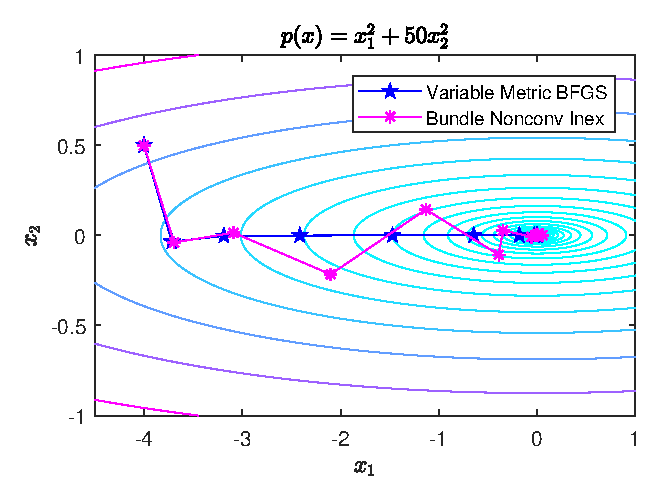
\includegraphics[width=\textwidth]{Pictures/Plots/final_parab.eps}
		%\subcaption{}
		%Parabola, \(kappa = 2\), sequwnces of \(x_{hats}\); Noll:\(10|1\), Hare: \(28|12\)
	\end{subfigure}
	\begin{subfigure}[t]{0.49\textwidth}
			%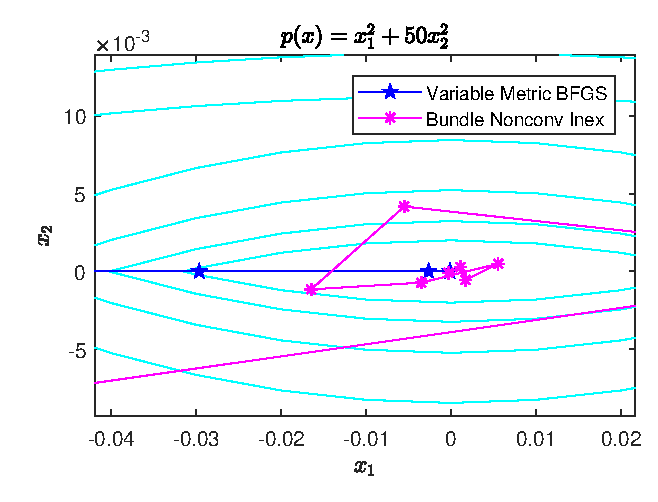
\includegraphics[width=\textwidth]{Pictures/Plots/final_parab_detail.eps}
			%\subcaption{detail, many steps of Hare in the end}
	\end{subfigure}
	\caption{Sequences of serious steps constructed by the proximal bundle algorithm and the variable metric algorithm respectively on the level lines of parabola \(p\). The right image is a detail of the plot on the left.\\
	Step size parameter: \(\kappa_+ = 2\) for both algorithms.}
	\label{fig_contour_parab}
\end{figure}

The second test function is a nonsmooth version of the above parabola. The function is given by 
\[ p_n(x): \R^2 \to \R, \quad x \mapsto \frac{1}{2}\Langle x, Ax \Rangle + \frac{1}{2}|x_1|+25|x_2|. \]

Due to the kink along the \(x_1\)-axis the curvature information supplied by \(Q_k\) is less reliable than for the smooth parabola.
Figure \ref{fig_contour_nonsm_parab} shows the sequences constructed by the two algorithms. Still the sequence provided by the variable metric algorithm does less zig-zagging than the one coming from the proximal bundle algorithm.
It is interesting to note, that the sequence provided by the proximal bundle algorithm is the same for both functions. This is not the case for the sequence generated by the metric bundle algorithm because the second order information of the two objective functions is different.

\begin{figure}[H]
	\begin{subfigure}[t]{0.49\textwidth}
		%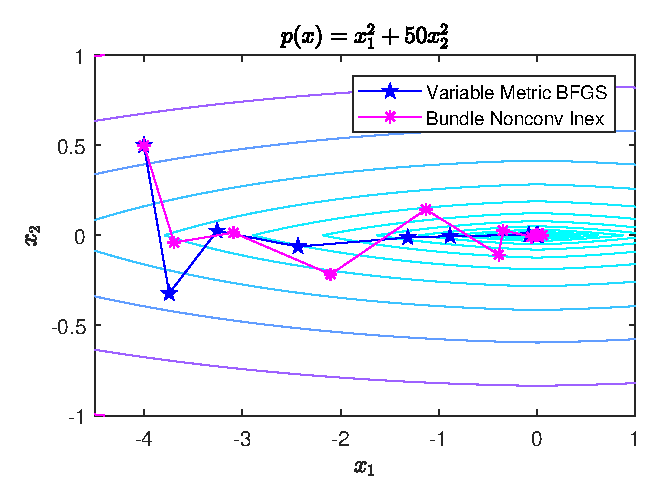
\includegraphics[width=\textwidth]{Pictures/Plots/final_nonsm_parab.eps}
		%\subcaption{Parabola, \(kappa = 2\), sequwnces of \(x_{hats}\); Noll:\(21|9\), same for adapted, Hare: \(28|12\)}
	\end{subfigure}
	\begin{subfigure}[t]{0.49\textwidth}
			%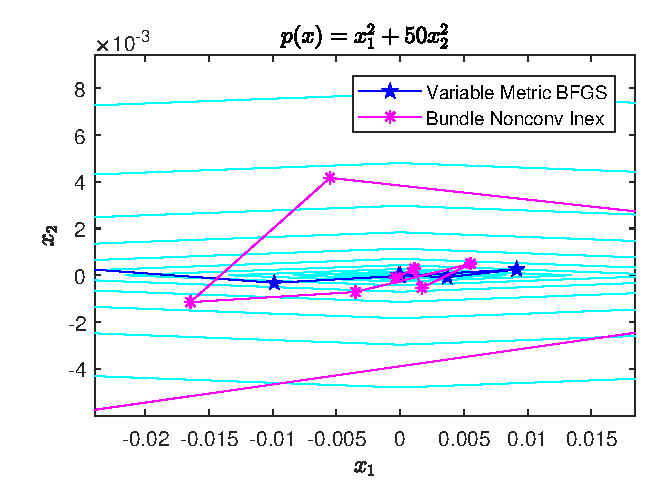
\includegraphics[width=\textwidth]{Pictures/Plots/final_nonsm_parab_detail.eps}
			%\subcaption{detail}
	\end{subfigure}
	\caption{Sequences of serious steps constructed by the proximal bundle algorithm and the variable metric algorithm respectively on the level lines of the nonsmooth quadratic function \(p_n\). The right image is a detail of the plot on the left.\\
	Step size parameter: \(\kappa_+ = 2\) for both algorithms.}
	\label{fig_contour_nonsm_parab}
\end{figure}

The bar plots in figures \ref{fig_bar_parab} and \ref{fig_bar_nonsm_parab} compare the accuracy of the solution and the number of steps that is needed by the different algorithms for the various noise forms. Here the nonconvex proximal bundle algorithm is compared to both variants of the variable metric method.

To address the random nature of the noise the tests are performed 20 times and the results averaged. The number of steps is rounded to end up with integers.
%\textcolor{red}{adaptive Q has to be explained before, reference}\\

\begin{figure}[ht]
	\begin{subfigure}[t]{0.49\textwidth}
		%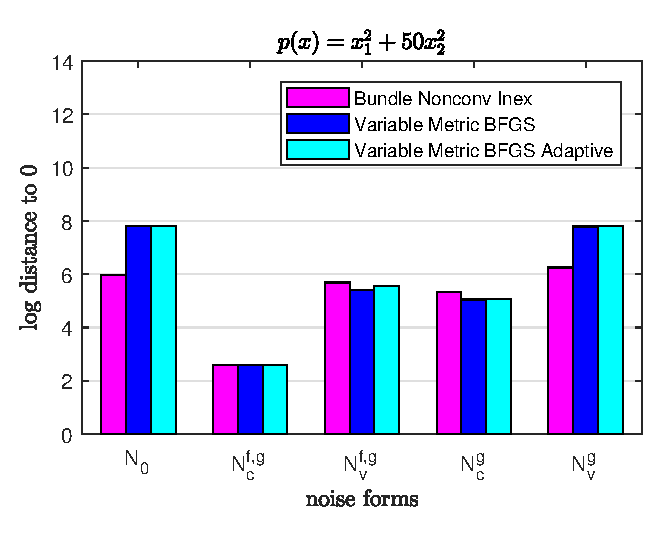
\includegraphics[width=\textwidth]{Pictures/Plots/accuracy_bar_parab_u_1-2.eps}
		%\subcaption{Parabola, \(kappa = 2\)}
	\end{subfigure}
	\begin{subfigure}[t]{0.49\textwidth}
			%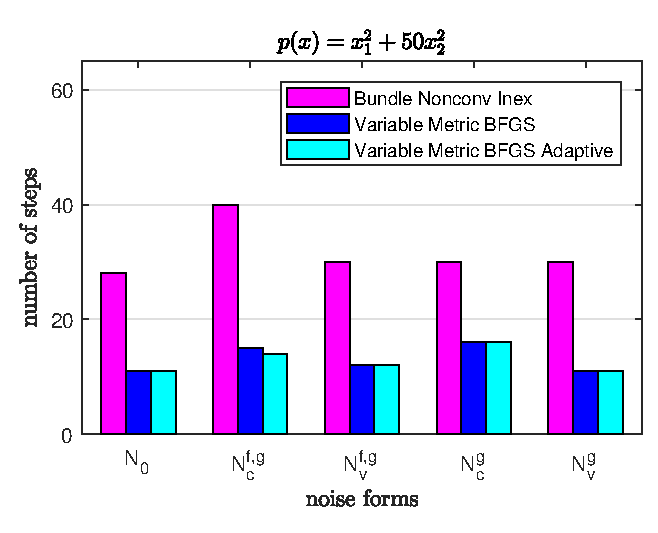
\includegraphics[width=\textwidth]{Pictures/Plots/steps_bar_parab_u_1-2.eps}
	%		\subcaption{}
	\end{subfigure}
	\caption{Left: Accuracy of the solution computed by the different versions of the variable metric bundle algorithm compared to the proximal bundle algorithm for the parabola \(p\) under different form of noise.\\
	Right: Comparison of the number of steps for the three algorithms.\\
	Step size parameters: \(\kappa_+ = 1.2\) for the proximal bundle method and \(\kappa_+ = 2\) for the variable metric algorithm. }
	\label{fig_bar_parab}
\end{figure}

In the smooth case one can see that the accuracy of the two algorithms is comparable. In the case where no noise is present and in the last case, which is the case with the least noise, the variable metric algorithm solves more accurately but for the proximal bundle algorithm the actually computed optimal value is still above the chosen tolerance of \(10^{-6}\).
In the cases of the more involved noise the accuracy is less.

A significant difference can be seen between the needed number of steps of the different algorithms. Here the variable metric versions of the bundle method can take advantage of the curvature information and the fact that for the smooth parabola the BFGS update approximates the Hessian matrix very well.
The difference in steps between the two update variants of the variable metric algorithm is neglectable and could also be present due to the random noise. This is what we expect as the scaling mechanism should not be invoked in the smooth case.

\begin{figure}[ht]
	\begin{subfigure}[t]{0.49\textwidth}
		%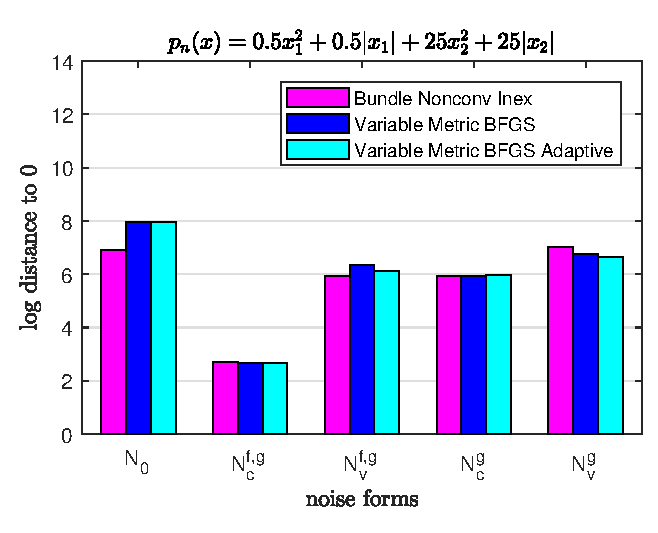
\includegraphics[width=\textwidth]{Pictures/Plots/accuracy_bar_nonsm_parab_u_1-2.eps}
		%\subcaption{Parabola, \(kappa = 2\)}
	\end{subfigure}
	\begin{subfigure}[t]{0.49\textwidth}
			%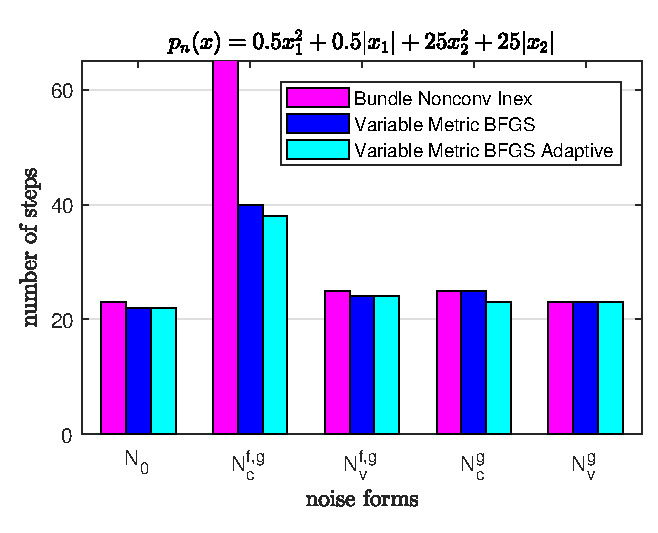
\includegraphics[width=\textwidth]{Pictures/Plots/steps_bar_nonsm_parab_u_1-2.eps}
			%\subcaption{}
	\end{subfigure}
	\caption{Left: Accuracy of the solution computed by the different versions of the variable metric bundle algorithm compared to the proximal bundle algorithm for the nonsmooth quadratic function \(p_n\) under different form of noise.\\
	Right: Comparison of the number of steps for the three algorithms. The left bar for the number of steps in the case of constant noise is cropped.\\
	Step size parameters: \(\kappa_+ = 1.2\) for the proximal bundle method and \(\kappa_+ = 2\) for the variable metric algorithm.}
	\label{fig_bar_nonsm_parab}
\end{figure}

In the nonsmooth case (shown in figure \ref{fig_bar_nonsm_parab}) the accuracy of all algorithms is very similar. The difference in the number of steps is now very small as well.
Only in the case of constant noise the proximal bundle algorithm performs rather badly. Here the number of steps is extremely large (over 250) in order to gain the same accuracy as the other algorithms.
The difference between the two update versions of the variable metric algorithm is still very small. It seems that the different scaling strategies have only a minor influence on the algorithm for this kind of objective function. Other tests showed that for example the choice of the step size updating parameters \(\kappa_+, \kappa_-\) have a lot more influence on the algorithm than the tested updating strategies. This can be seen in figures \ref{fig_no_noise_comp}  and \ref{fig_const_noise_comp} and figures \ref{fig_van_noise_comp} to \ref{fig_van_grad_noise_comp_large} in the appendix.


%\textcolor{red}{Noise form \(\text{N}_{\text{v}}^{\text{g}}\) is the one that is most similar to no noise; one can see: gradient noise has not as much impact as inexact function value (makes sense because only calculating with subgradients) -> in those cases variable metric algorithm more exact, but all over desired tolerance
%in terms of exactness proximal bundle algorithm slightly better, but not much; the two variants of the variable metric algorithm are more or less the same.\\
%for step sizes> proximal bundle algorithm needs a lot more steps than variable metric especially in the case of constant function value and gradient noise}

%\textcolor{red}{Figure \ref{fig_bar_nonsm_parab}:  in nonsmooth case accuracy of proximal bundle algorithm overall slightly better; need generally more steps, numbers of steps more equal apart from constant noise part where for a minor gain of accuracy a really high numer of steps is done (plot is cropped, really: over 250 steps)\\
%bigger difference if changing \(\kappa_+\) -> add plot for that and comment???}


%\textcolor{red}{second example: nonsmooth version of the parabola
	%\[ p: \R^2 \to \R, \quad x \mapsto \Langle x, \frac{1}{2}Ax\Rangle + 0.5 |x_1|+25|x_2|\]
	%kink makes problem with second order information; different possibilities\\
	%\begin{enumerate}
		%\item change nothing, just make sure \(Q_k\) bounded
		%\item scale \(Q_k\) if it becomes too big \\
		%advantage: not so much wrong information due to ``krummungs-Paradoxon''\\
		%drawback: everything scaled -> direction wrong if kink only in one direction; have to decide when \(Q_k\) too big, because exiist functions with high curvature
		%\item change only eigenvalue that got too high; check Change relative to last \(Q_k\) and stepsize
		%\item bigger stepsizes?
	%\end{enumerate}
	%first and third variants make sense in example}
%\textcolor{red}{tested in two ways; compared to Hare-Algortihm\\
%first plots with.. functions like in paper, then invetigated in more detail for which functions \(Q\) is of advantage\\}

%\textcolor{red}{
%\begin{itemize}
%	\item Vergleich mit Hare Version
%	\item Genauigkeit
%	\item Geschwindigkeit
%\end{itemize}}

%\textcolor{red}{recht gute Ergebnisse mit \(\frac{1}{k}Q_k\)\\
%ohne \(\frac{1}{k}\) eta extrem gross; mit: eta wird auch gross: 1e10}

%\textcolor{red}{In this section the above variant of an inexact bundle algorithm is compared with the nonconvex inexact bundle algorithm by Hare et al. in \cite{Hare2016}.\\
%For reasons of comparability the setting was chosen as in \cite{Hare2016}.\\
%The parameter set was chosen as follows: \(m = 0.05\), \(\gamma = 2\), \(t_1 = 0.1\) and the scaling parameters for the choice of \(t_k\) are \(\kappa_{+}=1.2\) and \(\kappa_{-}=0.8\) with the minimum possible \(t\) being \(t_{min}=0.03\).
%For the choice of the new bundle the information of the current prox-center and all elements with \(\alpha > 10^{-15}\) were kept in the bundle.
%As stopping condition  
%\[ \delta < \mathtt{tol}(1+f_{hat}) \]
%was used.
%If this did not apply within \(\max(300,205n)\) steps the algorithm also stopped.}

\subsubsection{Test Examples in Higher Dimensions}
\label{sec_num_test_ferr}

For the second test, which involves testing the performance of the different algorithms in different dimensions, the Ferrier polynomials are chosen as objective functions. These nonsmooth and nonconvex functions have already been used in \cite{Hare2010} and \cite{Hare2016}. The polynomials are constructed in the following way:

For \(i = 1,...,n\) we define 

\begin{align*}
	h_i: \R^n \to \R, \quad h(x) = (ix_i^2-2x_i)+\sum_{j=1}^n x_j.
\end{align*}

These functions are used to define

\begin{align*}
	f_1(x) &:= \sum_{i=1}^n |h_i(x)|, \\
	f_2(x) &:= \sum_{i=1}^n (h_i(x))^2, \\
	f_3(x) &:= \max_{i \in \{1,...,n\}}|h_i(x)|, \\
	f_4(x) &:= \sum_{i=1}^n \vert h_i(x)\vert+\frac{1}{2}\Vert x\Vert^2 \text{ and} \\
	f_5(x) &:= \sum_{i=1}^n \vert h_i(x)\vert+\frac{1}{2}\Vert x\Vert.
\end{align*}

%\textcolor{red}{plots of graphs???}

The graphs of the Ferrier polynomials for \(x \in \R^2\) are shown in figure \ref{fig_ferr_pol}.

\begin{figure}[ht]%
	\begin{subfigure}[t]{0.32\textwidth}
		%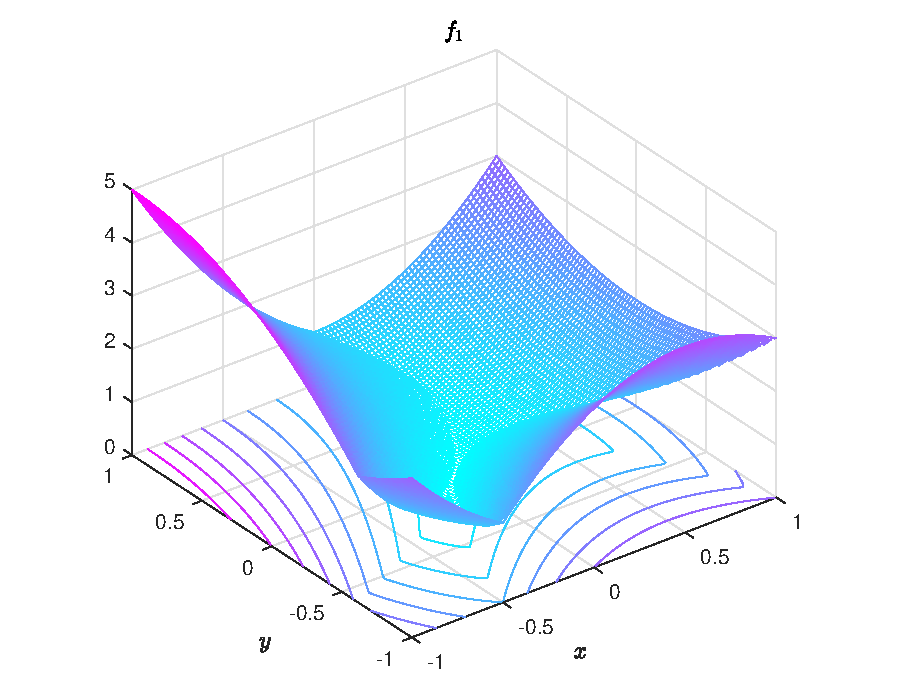
\includegraphics[width=\textwidth]{Pictures/Plots/testfun_f1.eps}
	\end{subfigure}
	\begin{subfigure}[t]{0.32\textwidth}
		%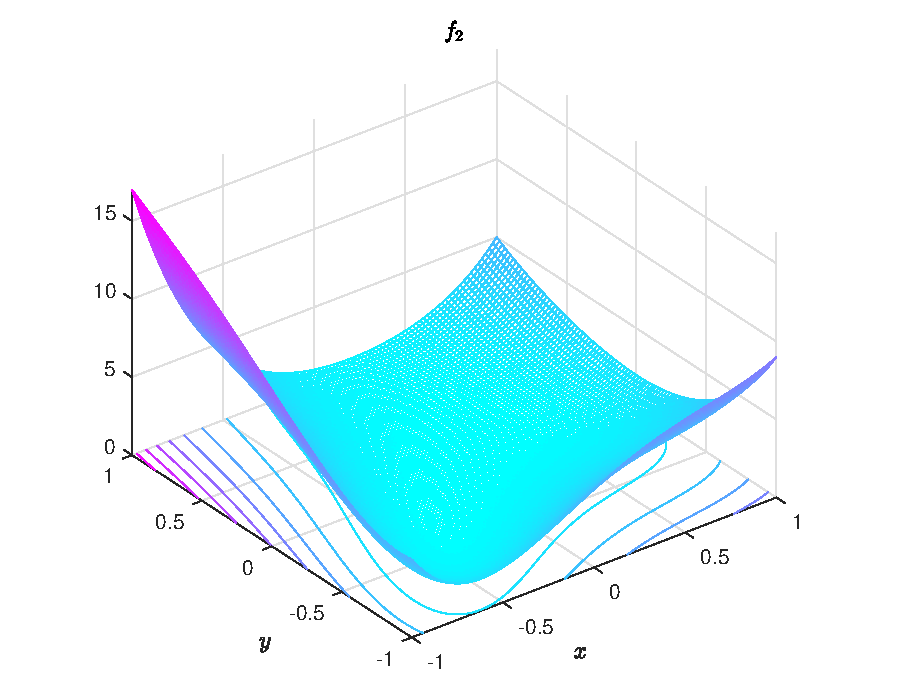
\includegraphics[width=\textwidth]{Pictures/Plots/testfun_f2.eps}
	\end{subfigure}
	\begin{subfigure}[t]{0.32\textwidth}
		%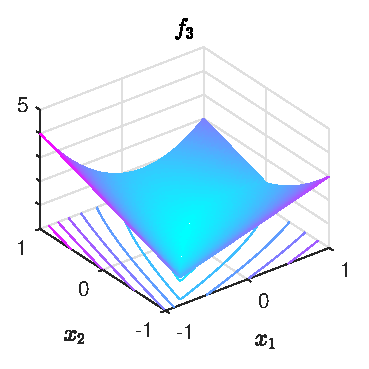
\includegraphics[width=\textwidth]{Pictures/Plots/testfun_f3.eps}
	\end{subfigure}
	\newline
	\begin{subfigure}{0.47\textwidth}
		\begin{flushright}
		%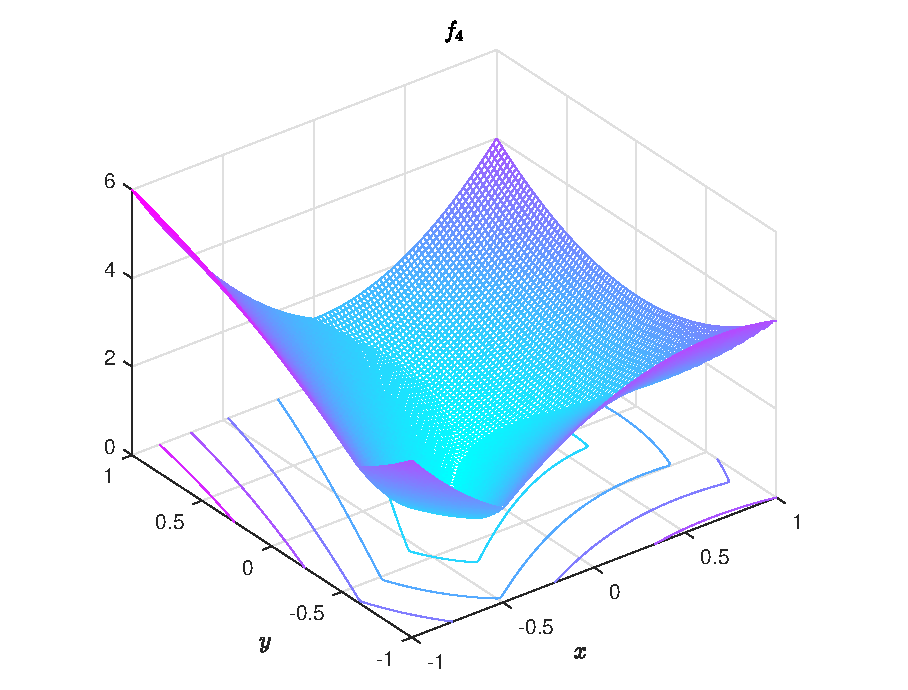
\includegraphics[width=0.68\textwidth]{Pictures/Plots/testfun_f4}
		\end{flushright}
		\vfil
	\end{subfigure}
	\begin{subfigure}{0.49\textwidth}
		%\begin{flushleft}
		%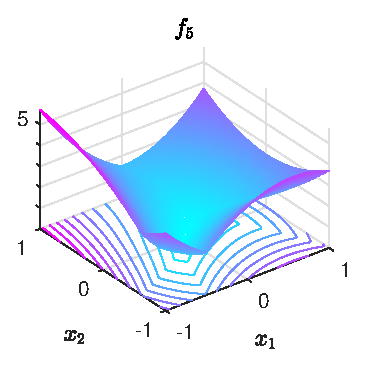
\includegraphics[width=0.65\textwidth]{Pictures/Plots/testfun_f5}
		%\end{flushleft}
	\end{subfigure}
	\caption{Graphs of the testfunctions $f_1$ to $f_5$ for $x\in\R^2$}
	\label{fig_ferr_pol}
\end{figure}

Ferrier polynomials are nonconvex, nonsmooth (except for \(f_2\)) and lower-\(\mathcal{C}^2\). They all have \(0\) as a global minimizer \cite[p. 23]{Hare2016}. The compact constraint set is \(X=\{x \in \R^n|\lvert x_i\rvert \leq 10, i = 1,...,n \}\).

The five test functions \(f_1\) to \(f_5\) are optimized for the dimensions \(n=\{2,3,...,15\} \cup \{20,25,30,40,50\}\).
The starting value for each test problem is \(x^1=[1,\frac{1}{4},\frac{1}{9},...,\frac{1}{n^2}]^{\top}\).

For the tests the step size of all algorithms is updated with \(\kappa_+ = 1.2\), which provided better results for these specific test functions.

The accuracy measures absolute logarithmic distance to the global minimum. In case that the algorithm finds a local minimum, which is possible for nonconvex objective functions, this lowers the accuracy.


\begin{figure}[ht]%
	\begin{subfigure}{0.49\textwidth}
		%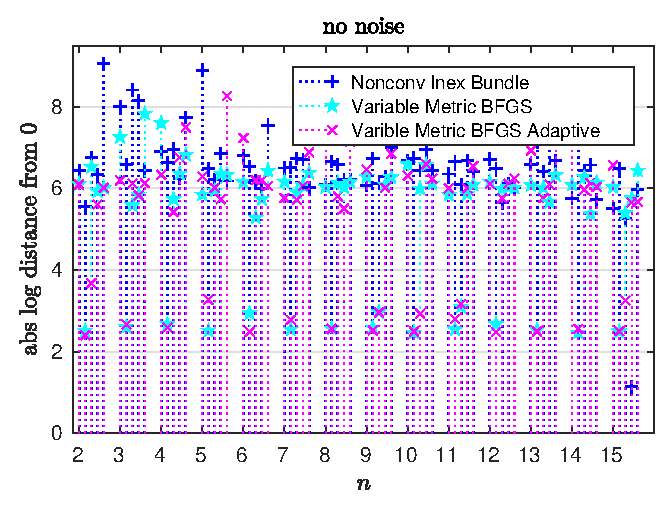
\includegraphics[width=\textwidth]{Pictures/Plots/no_noise.eps}%
	\end{subfigure}
	\begin{subfigure}{0.49\textwidth}
		%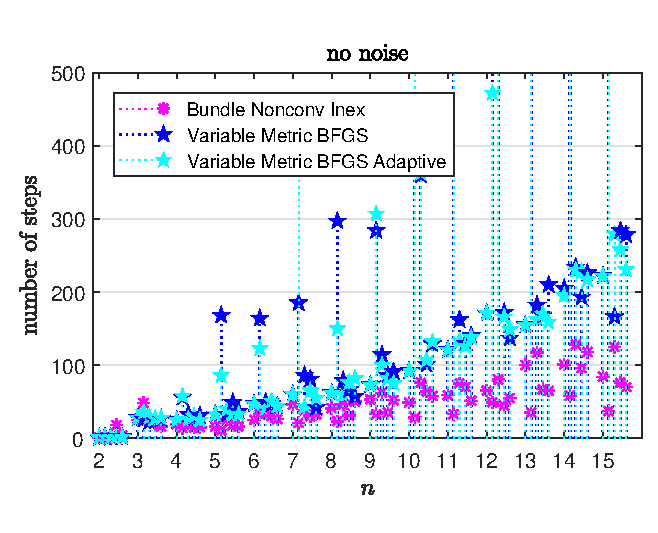
\includegraphics[width=\textwidth]{Pictures/Plots/steps_no_noise.eps}%
	\end{subfigure}
	\caption{Comparison of accuracy and number of steps for the proximal bundle algorithm and the variable metric bundle algorithm in the case of no noise.}
	\label{fig_no_noise}
\end{figure}

In the figures \ref{fig_no_noise} to \ref{fig_van_noise} and \ref{fig_const_grad_noise} to \ref{fig_van_grad_noise_large} in the appendix the achieved accuracy and the needed number of steps are shown for the proximal bundle method and two versions of the variable metric method.

Figure \ref{fig_no_noise} shows the situation if no noise is present and can be seen as a benchmark for the other noise forms.
It is clearly visible that the desired accuracy of \(10^{-6}\) is not always achieved by the different algorithms. A reason for this is that the objective functions have several local minima where the algorithms can get stuck. It seems that this happens more seldom to the proximal bundle algorithm than the variable metric method.

For the Ferrier polynomials the proximal bundle algorithm needs significantly less steps than the variable metric algorithm. It can also be observed that the cases where the variable metric algorithm is stuck in a local minimum, the number of steps needed rises significantly. This is not the case for the proximal bundle algorithm.

The performance of the two variants of the two versions of the variable metric method are similar. It seems however as if the adaptive version performed slightly better in terms of the number of steps used.


\begin{figure}[ht]
	\begin{subfigure}{0.49\textwidth}
		%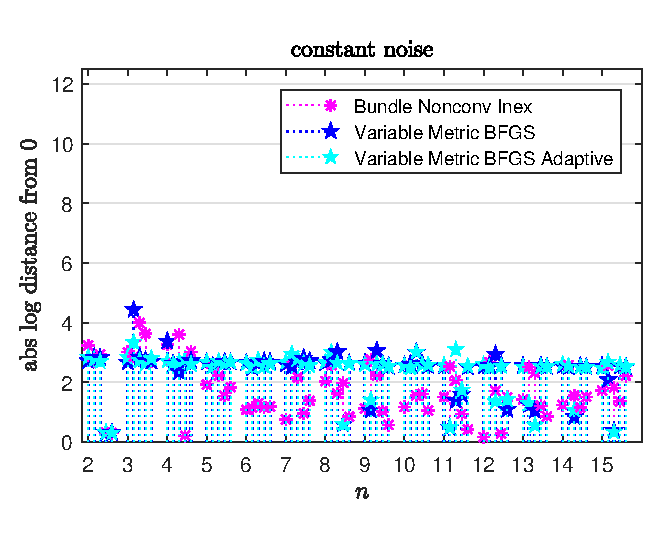
\includegraphics[width=\textwidth]{Pictures/Plots/constant_noise.eps}%
	\end{subfigure}
	\begin{subfigure}{0.49\textwidth}
		%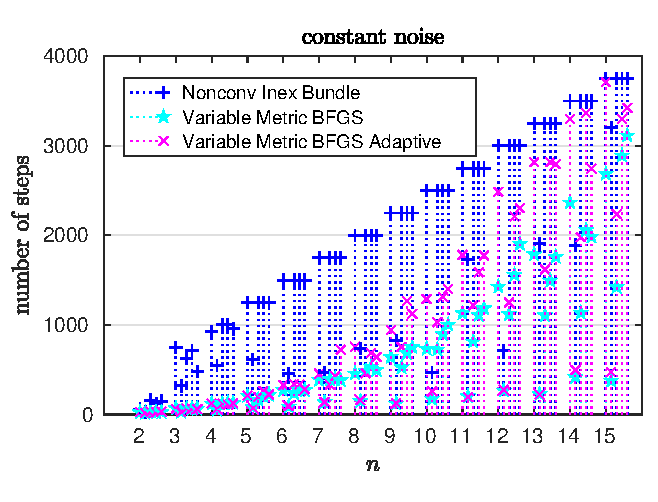
\includegraphics[width=\textwidth]{Pictures/Plots/steps_constant_noise.eps}%
	\end{subfigure}
	\caption{Comparison of accuracy and number of steps for the proximal bundle algorithm and the variable metric bundle algorithm in the case of constant noise}%
	\label{fig_const_noise}%
\end{figure}

In the case of constant noise the variable bundle methods perform better than the proximal version. They are more stable in the achieved accuracy and need considerably less steps than the other method.

\begin{figure}[ht]
	\begin{subfigure}{0.49\textwidth}
		%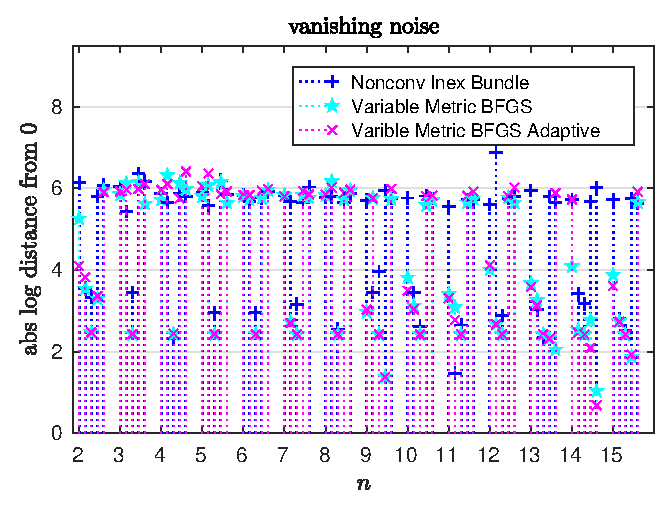
\includegraphics[width=\textwidth]{Pictures/Plots/vanishing_noise.eps}%
	\end{subfigure}
	\begin{subfigure}{0.49\textwidth}
		%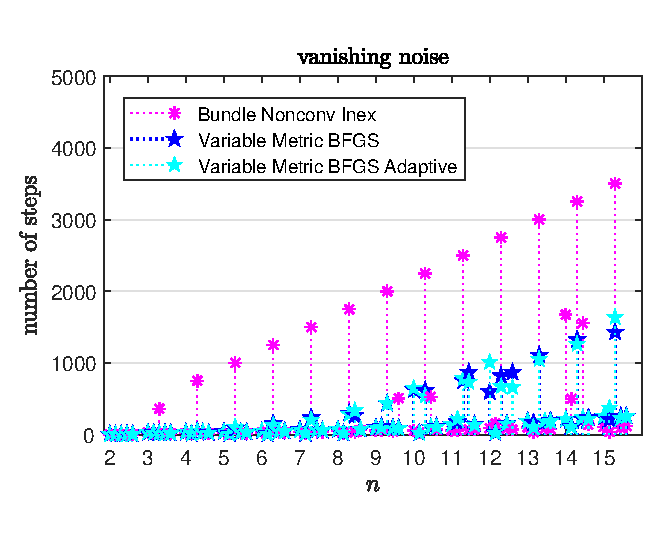
\includegraphics[width=\textwidth]{Pictures/Plots/steps_vanishing_noise.eps}%
	\end{subfigure}
	\caption{Comparison of accuracy and number of steps for the proximal bundle algorithm and the variable metric bundle algorithm in the case of vanishing noise}%
	\label{fig_van_noise}%
\end{figure}

For the other noise forms the three algorithms perform similar in terms of the accuracy but the variable bundle methods need consistently more steps.
The only exception from this is case of vanishing noise. Here the proximal bundle method needs extremely many more steps  than the variable metric bundle method to optimize function \(f_3\). This shows that the performance of the different algorithms depend on both the form of noise and the specific objective function.

The plots for the higher dimensional data \(x \in \R^n\) for \(n = \{20,25,30,40,50\}\) are included in the appendix (figures \ref{fig_no_noise_large} to \ref{fig_van_grad_noise_large}).
Also in higher dimensions the algorithms achieve a similar accuracy. The number of steps needed for convergence in generally higher, but still the proximal bundle method needs less steps in most situations.
In the cases where there is noise on the function value, the algorithms almost always stop because the maximum number of steps is reached. The only exception is the smooth function \(f_2\). Here the variable  metric methods perform a lot better  than the proximal bundle algorithm in terms of the number  of steps, because the curvature information is more reliable.

Finally the influence of the step size updating parameter \(\kappa_+\) is shown and the performance of the hybrid method.
This last method, denoted by 'Variable Metric BFGS, \(k\)-scaled' in the figures, uses the scaled BFGS update for the metric matrix \(Q_k\) and then scales this matrix again by the step size. This means the final matrix is \(Q_k = \frac{1}{k}\tilde{Q}_k\) if \(\tilde{Q}_k\) denotes the matrix after the scaled BFGS update, lowering the influence of the metric matrix in each serious step.
In this way the method starts out as the variable metric method and then behaves more and more like the proximal bundle method.

This shows that the additional curvature information can make a considerable difference in the convergence speed, especially for matrices \(Q_k\) that model the behavior of the objective function at the kinks correctly.
It is therefore an interesting but still open question if such matrix updates can be found.

The algorithms used for the comparison of the different \(\kappa_+\) are endowed with the scaled BFGS update from section \ref{update_1}. The parameters \(\kappa_+ = 1.2\) and \(\kappa_+ = 2\) are compared.
Here only the exact case and the case of constant noise for the lower dimensions are depicted in figure \ref{fig_no_noise_comp} and \ref{fig_const_noise_comp}. The situation for the other noise forms is shown in figures \ref{fig_van_noise_comp} to \ref{fig_van_grad_noise_comp_large}  in the appendix.

\begin{figure}[ht]%
	\begin{subfigure}{0.49\textwidth}
		%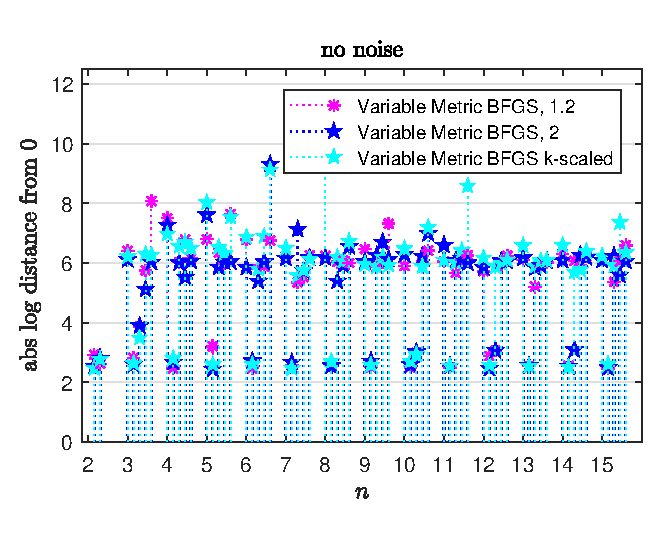
\includegraphics[width=\textwidth]{Pictures/Plots/no_noise_comp.eps}%
	\end{subfigure}
	\begin{subfigure}{0.49\textwidth}
		%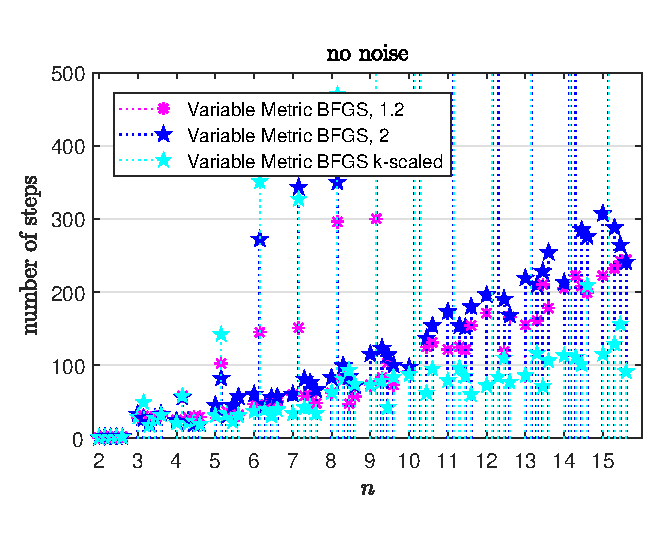
\includegraphics[width=\textwidth]{Pictures/Plots/steps_no_noise_comp.eps}%
	\end{subfigure}
	\caption{Influence of the step size updating parameter \(\kappa_+ = 1.2\) and \(\kappa_+ =2 \) and performance of the hybrid method in the exact case. The reached accuracy is depicted on the left, the needed number of steps on the right.}
	\label{fig_no_noise_comp}
\end{figure}

\begin{figure}[ht]%
	\begin{subfigure}{0.49\textwidth}
		%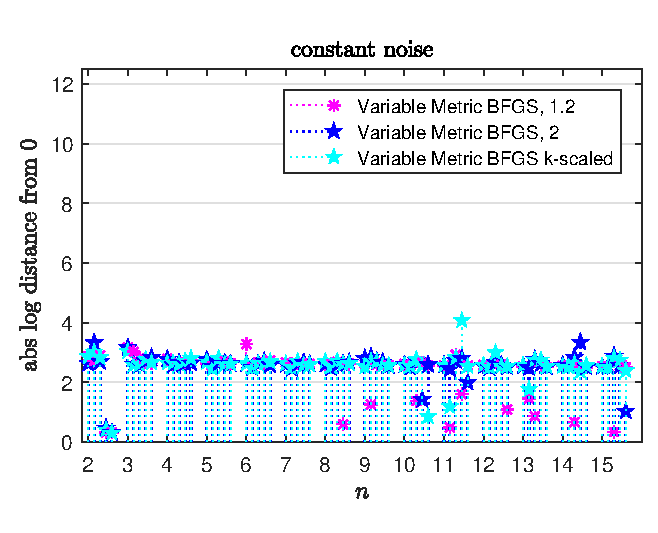
\includegraphics[width=\textwidth]{Pictures/Plots/constant_noise_comp.eps}%
	\end{subfigure}
	\begin{subfigure}{0.49\textwidth}
		%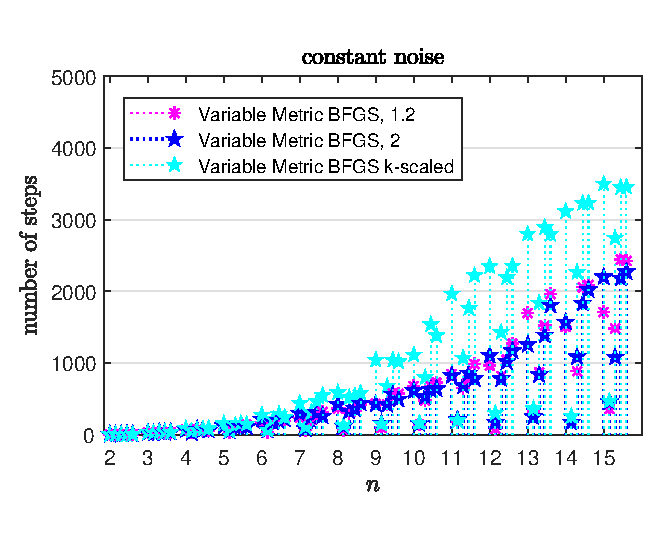
\includegraphics[width=\textwidth]{Pictures/Plots/steps_constant_noise_comp.eps}%
	\end{subfigure}
	\caption{Influence of the step size updating parameter \(\kappa_+ = 1.2\) and \(\kappa_+ =2 \) and performance of the hybrid method for constant noise. The reached accuracy is depicted on the left, the needed number of steps on the right.}
	\label{fig_const_noise_comp}
\end{figure}


One can see that contrary to the academic test example, where the choice \(\kappa_+ = 2\) gives better results for the number of steps, here the parameter \(\kappa_+=1.2\) performs better.
In the case of constant noise the numbers of steps are similar.
As  expected the accuracy of the two methods is very similar, because only one parameter is changed. The number of steps shows however that parameter tuning can be useful. Here it is important to keep in mind that the optimal parameter depends on the objective function and the noise form.

The performance of the hybrid method is, as can be expected, similar to the proximal bundle method. As the scaling is quite strong the influence of the metric matrix decreases rather quickly.
This means that in cases where the proximal bundle method performed better, the same is true for the hybrid method. The increase in the number of steps is only minor. Likewise in the case of constant noise (figure \ref{fig_const_noise_comp}) for example, where the proximal bundle method needed a lot of steps, these steps are also needed by the hybrid method. Two advantages of the hybrid method still come into play for this noise form: The significant decrease in the number of steps starts only in higher dimensions, where the total number of steps grows larger. Here a 'slower' scaling could yield even better numbers.
The other advantage is the more stable accuracy. This holds true for all dimensions.
%
%
%\textcolor{red}{say where plots left and right...}
%
%%\subsection{Subproblem Variable Metric}
%%
%%For comparision: Subproblem proximal bundle
%%
%%\begin{align}
	%%&\min_{d \in \R^n, \xi \in \R} \xi + \frac{1}{2t_k}\|d\|^2 = \xi + \frac{1}{2}d^{\top}\left(\frac{1}{t_k}\mathbf{I}\right)d \\
	%%&\text{s.t.} \quad f(\hat{x}^k)+{g^j}^{\top}d - e^k_j - \xi \leq 0, \quad j \in J_k
%%\end{align}
%%
%%Subproblem variable metric:
%%\begin{align}
	%%&\min_{d \in \R^n, \xi in \R} \xi + \frac{1}{2}d^{\top}D_kd \\
	%%&\text{s.t.} \quad f(\hat{x}^k)+{g^j}^{\top}d - e^k_j - \xi \leq 0, \quad j \in J_k
%%\end{align}
%%These are \(\R^{n+1}\) dimensional quadratic optimization problems.\\
%%
%%\textcolor{red}{Find out if \(D_k\) is diagonal matrix! Think not.} \\
%%
%%Approaches not so different. Instead of just scaling the identity \(\rightarrow\) induce ``curvature information'' via past subgradients. \\
%%
%%Dual proximal subproblem:
%%\begin{align}
	%%&\min_{\alpha \in \R^{|J_k|}} \frac{1}{2} \left(\sum_{j \in J_k}{\alpha_jg^j}\right)^{\top} t_k\mathbf{I} \left(\sum_{j \in J_k}{\alpha_jg^j}\right) + \sum_{j \in J_k}{\alpha_j e_j^k} \\
		%%&\text{s.t.} \quad \sum_{j \in J_k}{\alpha_j} = 1 \text{ and } \alpha_j \geq 0 ~ j \in J_k
%%\end{align}
%%
%%
%%Dual variable metric subproblem:
%%\begin{align}
	%%&\min_{\alpha \in \R^{|J_k|}} \frac{1}{2} \left(\sum_{j \in J_k}{\alpha_jg^j}\right)^{\top} D^{-1}_k \left(\sum_{j \in J_k}{\alpha_jg^j}\right) + \sum_{j \in J_k}{\alpha_j e_j^k} \\
		%%&\text{s.t.} \quad \sum_{j \in J_k}{\alpha_j} = 1 \text{ and } \alpha_j \geq 0 ~ j \in J_k
%%\end{align}
%%
%%These are \(\R^{|J_k|}\) dimensional quadratic optimization problems. \\
%%
%%\textcolor{red}{check linear independent \(g^j\)'s.}
%
%\begin{itemize}
	%\item Hare Algo seems to be better in ``global'' optimization \\
	%Noll seems to get stuck in local Minima more often
	%\item different ``Versions'' of Noll: Q ``ignored'' near kinks because there no curvature, but seems be be ``infinite''
	%\item the t-update Parameter has A LOT of influence on the performance of the algorithm
%\end{itemize}